\chapter{Experimental Setup}

This section discusses practical considerations related to the experiments undertaken in this dissertation. The important details of the hand tracking system used are discussed in Section \ref{sec:htm}. The details of the nature of the real dataset used in this dissertation are described in Section \ref{sec:es:msradset}. The performance metric of the hand tracking system used is defined in Section \ref{sec:pm}, this is particularly important as it is central to how the performance of a dataset is evaluated. Internal testing of the experimental setup is discussed in Section \ref{sec:sd:st}. Details of the experiments performed are discussed in Section \ref{es:exp}. Finally, miscellaneous matters are discussed in Section \ref{sec:sd:misc}.

\label{chap:es}
\section{Hand Tracking Model}
\label{sec:htm}
The V2V-Posenet model\cite{moon2018v2v} is used as the hand tracking system for training on, an overview of the network can be seen in Figure \ref{fig:v2vposenet}. It takes a depthmap $\bm{Z}$ as an input, and a 3D vector $\bm{v}$ denoting the centre of the hand in $\bm{Z}$ in 3D space. For this dissertation, where depthmap $\bm{Z}$ has an image resolution of $(a\times b)$, $\bm{v}_x = \frac{a}{2}$ and $\bm{v}_y=\frac{b}{2}$ and $\bm{v}_z = \bm{Z}_{\frac{a}{2},\frac{b}{2}}$. It outputs 3D predicted joints $\bm{\Phi}$ given a depthmap image $\bm{Z}$. Knowledge of the pipeline of this model is critical for generating the correct synthetic data. In the pipeline, the input depthmap is converted to a Point Cloud using $\bm{v}$ as a basis. In the context of this experiment, a Point Cloud is defined as an array of 3D vertices that describes the shape of an object in 3D space. Given that this is generated from a planar depth image, the Point Cloud does not define the entire surface of the hand. As such, self occlusions will also be visible in the Point Cloud. The algorithm for converting from a depthmap to a Point Cloud takes the indices of a pixel as an $x$, $y$ coordinate pair, and the value in that pixel as the $z$ coordinate. Points which are greater than a certain radius away from $\bm{v}$ are discarded, thus acting as a segmentation step between foreground and background. This Point Cloud is then turned into a voxel representation. Voxels are the 3D analogue to 2D pixels, and in the case of this setup, it is the 3D analogue to a 2D binary image. Formally, it is a 3D tensor, and can be seen as a verbose version of the Point Cloud.

An open source implementation of V2V-Posenet written in Python3 was used for this dissertation\footnote{\url{https://github.com/dragonbook/V2V-PoseNet-pytorch} (accessed 29th April 2020)}.

\section{MSRA Dataset}
\label{sec:es:msradset}
As previously mentioned, the MSRA dataset\cite{sun2015cascaded} is used as a baseline to compare the synthetic dataset. The MSRA dataset consists of depth images of nine subjects, and each subject performs seventeen gestures drawn from American Sign Language, to which there are approximately five-hundred frames each\footnote{\url{https://jimmysuen.github.io/txt/cvpr15\_MSRAHandGestureDB\_readme.txt} (accessed 29th April 2020)}. The dataset is split 90/10 for training and testing respectively. The implementation described in Section \ref{sec:htm} contains code for training on the MSRA dataset and it was not substantially modified.

\section{Performance Metrics}
\label{sec:pm}
\begin{figure}
    \centering
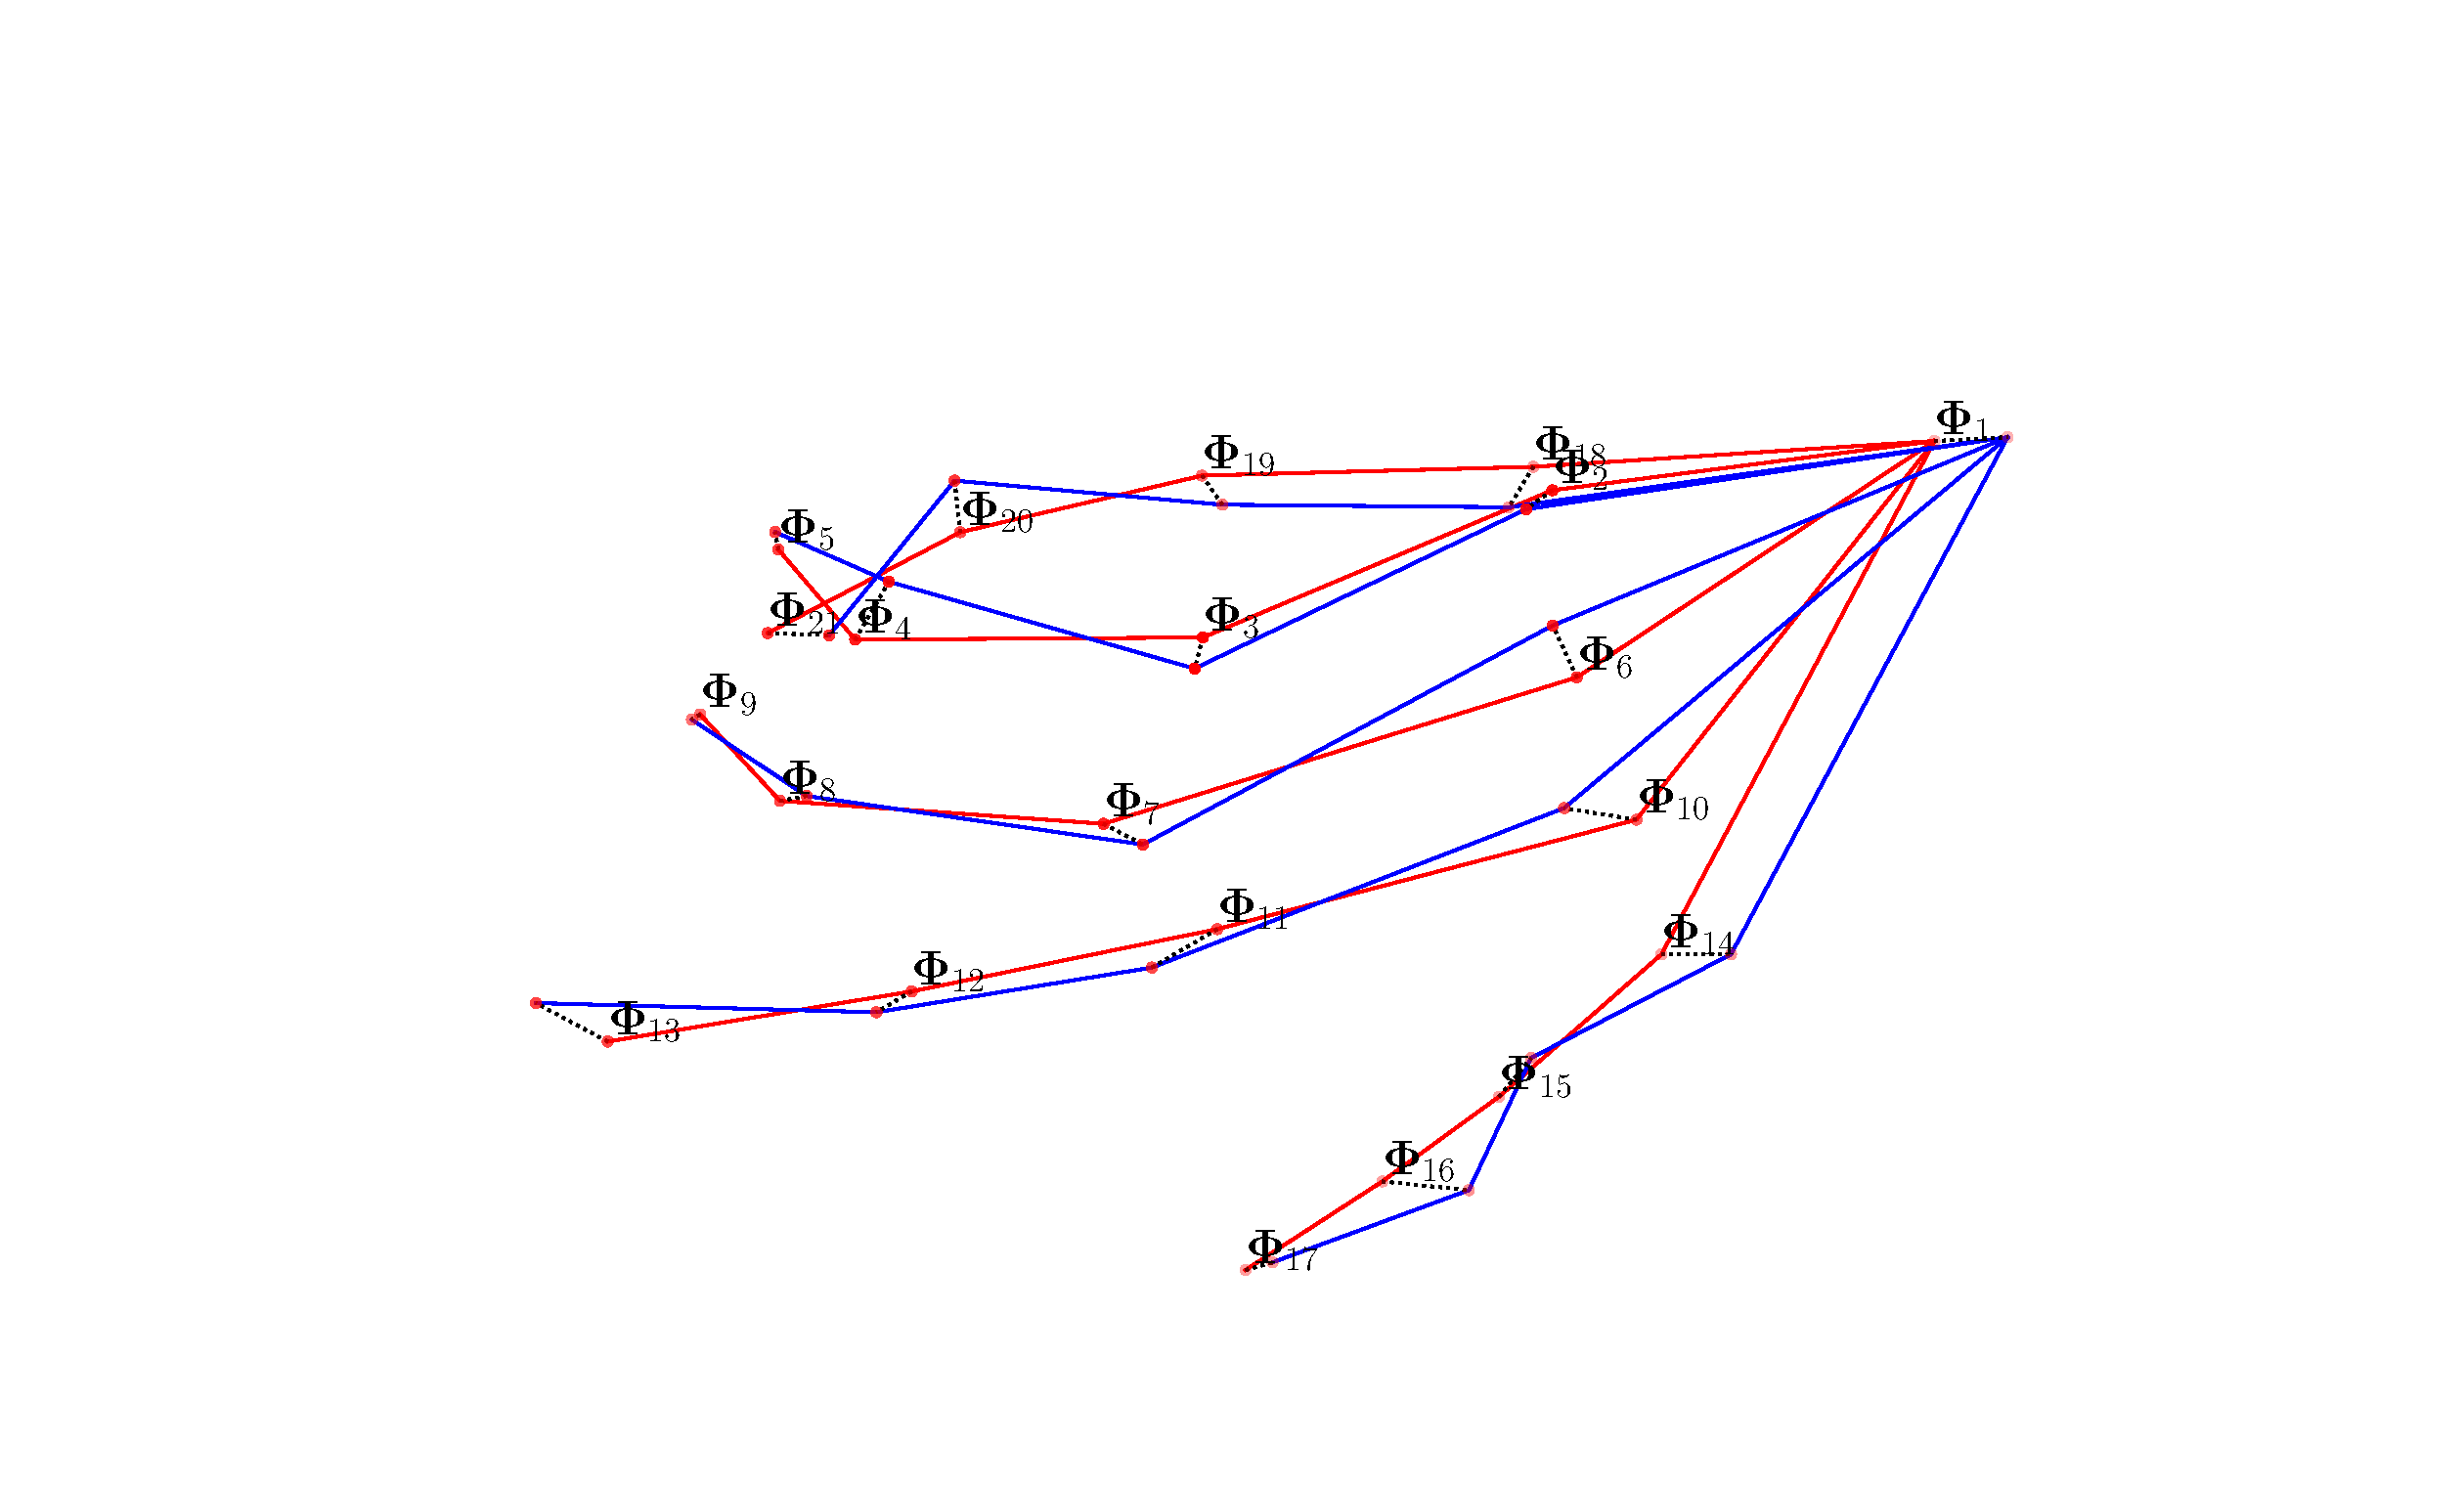
\includegraphics[width=0.8\linewidth]{figs/general/performance_metric.pdf}
\caption{A visualisation of the {\slshape Global Error} performance metric. The prediction and groundtruth are shown in blue and red respectively. The performance metric measures the average distance for each joint between the prediction and groundtruth, denoted for this example by the dotted black line. Each $\bm{\Phi}_{n}$ corresponds to a keypoint as in Figure \ref{fig:sd:hand}.}
\end{figure}
The performance metrics discussed in this section are the cornerstone from which synthetic data is compared with real data. As previously discussed, the goal of a hand tracking system is to extract information about a hand from an image of a hand, and one way of evaluating the hand tracking system's performance is by using the metrics described below. Therefore, the questions asked about synthetic hand data in this dissertation are answered using these metrics.

The primary performance metric used is mean per-joint error, as used in\cite{sun2015cascaded}. This performance metric shall be referred to as {\slshape Global Error}. Specifically, for {\slshape each joint}, the average euclidian distance (in millimeters) in 3D space is computed between the groundtruth keypoint $\bm{\mathrm{Y}}^{i}_{n,m}$ and predicted keypoint $\bm{\mathrm{Y}}^{o}_{n,m}$. An important implication of this is that the prediction could predict the correct articulation of the hand, but the per-joint error is still high because the global orientation or location of $\bm{\mathrm{Y}}^{i}_{n,m}$ is different to $\bm{\mathrm{Y}}^{o}_{n,m}$. The model must therefore aim to correctly predict orientation as well as articulation to perform well on this metric.

% \begin{equation}
%     d\Big(\bm{a}, \bm{b}\Big) = \sqrt{(\bm{a}_x-\bm{b}_x)^2+(\bm{a}_y-\bm{b}_y)^2+(\bm{a}_z-\bm{b}_z)^2}
% \end{equation}

There are $K$ images in the test dataset, and the hand tracking model predicts $N$ joints $\bm{\Phi}$ for each image $\bm{Z}$. $E^G$ is the average error for all joints, and $E^{G}_{n}$ denotes the average error for an individual joint $\bm{\Phi}_n$ (e.g. the per-joint error for the index MCP joint).
\begin{equation}
E^{G}_{n} = \frac{1}{K}\sum_{m=1}^{K} ||\bm{\mathrm{Y}}^{i}_{m,n} - \bm{\mathrm{Y}}^{o}_{m,n}||
\end{equation}
\begin{equation}
    E^{G} = \frac{1}{N}\sum_{k=1}^{N} E^{G}_{k}
\end{equation}

Through empirical observation, it was found that the V2V-Posenet model would often correctly predict the {\slshape articulation} and global {\slshape orientation} of the hand correctly, but not the global {\slshape position}. To account for situations where the model predicts the articulation and orientation correctly, but not the global position in 3D space, the following metric is also used. The above metric is modified by translating $\bm{\Phi}$ by the difference between the predicted and groundtruth values for the location of this wrist. This performance metric shall be referred to as {\slshape Local Error}. This means that the error for the wrist joint will be zero (thus this value is not reported in the local error metric). This second metric exists to provide more insight into performance. While the former metric is most important to optimise for a robust hand tracking system, this second metric can provide an intermediate goal to achieve in optimising the hand tracking model.

\begin{equation}
    E^{L}_{n} = \frac{1}{K}\sum_{m=1}^{K} ||\bm{\mathrm{Y}}^{i}_{m,n} + (\bm{\mathrm{Y}}^{o}_{m,n} + (\bm{\mathrm{Y}}^{i}_{m,0} - \bm{\mathrm{Y}}^{o}_{m,0}))||
\end{equation}
\begin{equation}
    E^{L} = \frac{1}{n}\sum_{k=1}^{N} E^{L}_{k}
\end{equation}

Typically, the scale that a hand lies within in local space is {\slshape approximately} $200mm$, that is the maximum span of an adult human hand. The precise value of this range is not important, but it does serve to illustrate how the above performance metrics are interpreted, particularly the second metric. For example, if the average per-joint error of one joint is $80mm$, that is far away, if it is $800mm$, then there is likely something very wrong with the system, and if it is $8mm$, that is perhaps a reasonable average error. There is no exact interpretation to this however, which is why a baseline exists to judge experimental results.

As discussed above, the MSRA dataset is used as the baseline for this experiment. The crux of this dissertation is to evaluate the merits of using synthetic data for training a hand tracking system. To answer this question, the V2V-Posenet model is trained and tested using the respective training sets of MSRA, which produces a particular error value. The answer is provided by comparing the performance of training the V2V-Posenet model with the MSRA dataset versus training it with the synthetic datasets.

% There are three datasets to consider, the existing MSRA dataset, as well as two datasets that I generate; non-deterministic and deterministic synthetic datasets generated using the MANO model. The two datasets that I generate are split into a training and test set in the same size and proportion to MSRA (67893 and 8498 respectively). For the baseline of this dissertation., the V2V-Posenet model is trained for five epochs with the MSRA training dataset, and validated on the equivalent test set. The error that this gives, based on the performance metric in Section \ref{sec:pm} is the baseline, and this forms the foundation from which the rest of the experiments are drawn. The goal of this dissertation is to asses.

\section{Software Testing}
\label{sec:sd:st}
Software testing is the primary method used for improving the synthetic data pipeline. Software testing for this dissertation and the evaluation of the merits of using synthetic data are two separate concerns. While the latter is evaluated using the performance metrics in Section \ref{sec:pm}, software testing refers to the performance of the internal components of the synthetic data generation system. The performance metric is directly reliant on the internal performance of this system, and the performance metric {\slshape might} suffer because of a bad design of the synthetic data pipeline, and not because my hypothesis about synthetic data is false. It is imperative that the synthetic data pipeline is optimal so that the performance metric in Section \ref{sec:pm} solely answers the hypothesis, and not a failing in my design of the pipeline. To address this concern, different tests were devised to evaluate the performance

In both the synthetic data generation pipelines, these are aspects that I believe are liable to failing.

\subsection{Data Visualisation}
\label{sec:es:st:dv}
\begin{figure}
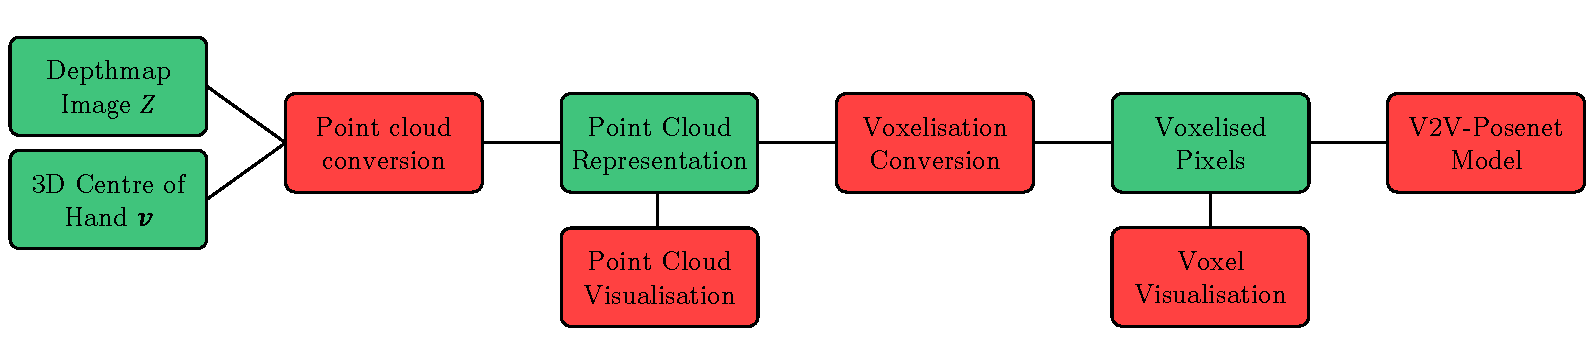
\includegraphics[width=\linewidth]{figs/general/voxelisation.pdf}
\caption{A diagram of the preprocessing steps for the V2V-Posenet model, from input depthmap image $\bm{Z}$ and centre $\bm{v}$ to voxels, this voxelised representation is then passed into the 3D CNN. The two red boxes for {\slshape Point Cloud Visualisation} and {\slshape Voxel Visualisation} denote the two visualisation stages described in Section \ref{sec:es:st:dv}.}
\label{fig:prevoxels}
\end{figure}
Visualisation served as the backbone of software testing in this dissertation. Ideally, unit testing or some other sort of numerical test would be used, but given the complicated nature of the data being handled, I am not aware of any reliable unit testing regimen. The following parts describe the individual visualisation tests that were performed.

\subsubsection{Depthmap Visualisation}
This step visualises the conversion of the mesh outputted by MANO into the depthmap, as well as the normalisation of this image. This step was important for seeing whether the camera was behaving as expected, as well as visualising the domain of the foreground pixels and ensuring that there is a clear boundary between these foreground pixels and the background. Examples can be seen in Figure \ref{fig:sd:nd} and Figure \ref{fig:sd:d}.

\subsubsection{Pointcloud Visualisation}
The conversion of the depthmap to the pointcloud it one of the most important steps in the pipeline. An example of this can be seen in Figure \ref{fig:es:pc}. As previously described, the step of converting the depthmap to a Point Cloud uses a 3D centre point as a reference to the `centre' $\bm{v}$ of the hand, and all points further than a certain distance to this point are discarded. In Figure \ref{fig:es:pc}, this centre is denoted by the confluence of the three thin red lines. The threshold in which points beyond $\bm{v}$ are discarded is denoted by the green sphere. The purpose of this step is to ensure that most points lie within this green sphere. The definition of {\slshape most} is defined by my empirical observation of the MSRA dataset visualised at this step. It was found that {\slshape most}, but not all points describing the hand lie within this green sphere. The parameters that can be optimised in this step are the centre point of the image. This step was implemented with {\slshape Matplotlib}.

\begin{figure}
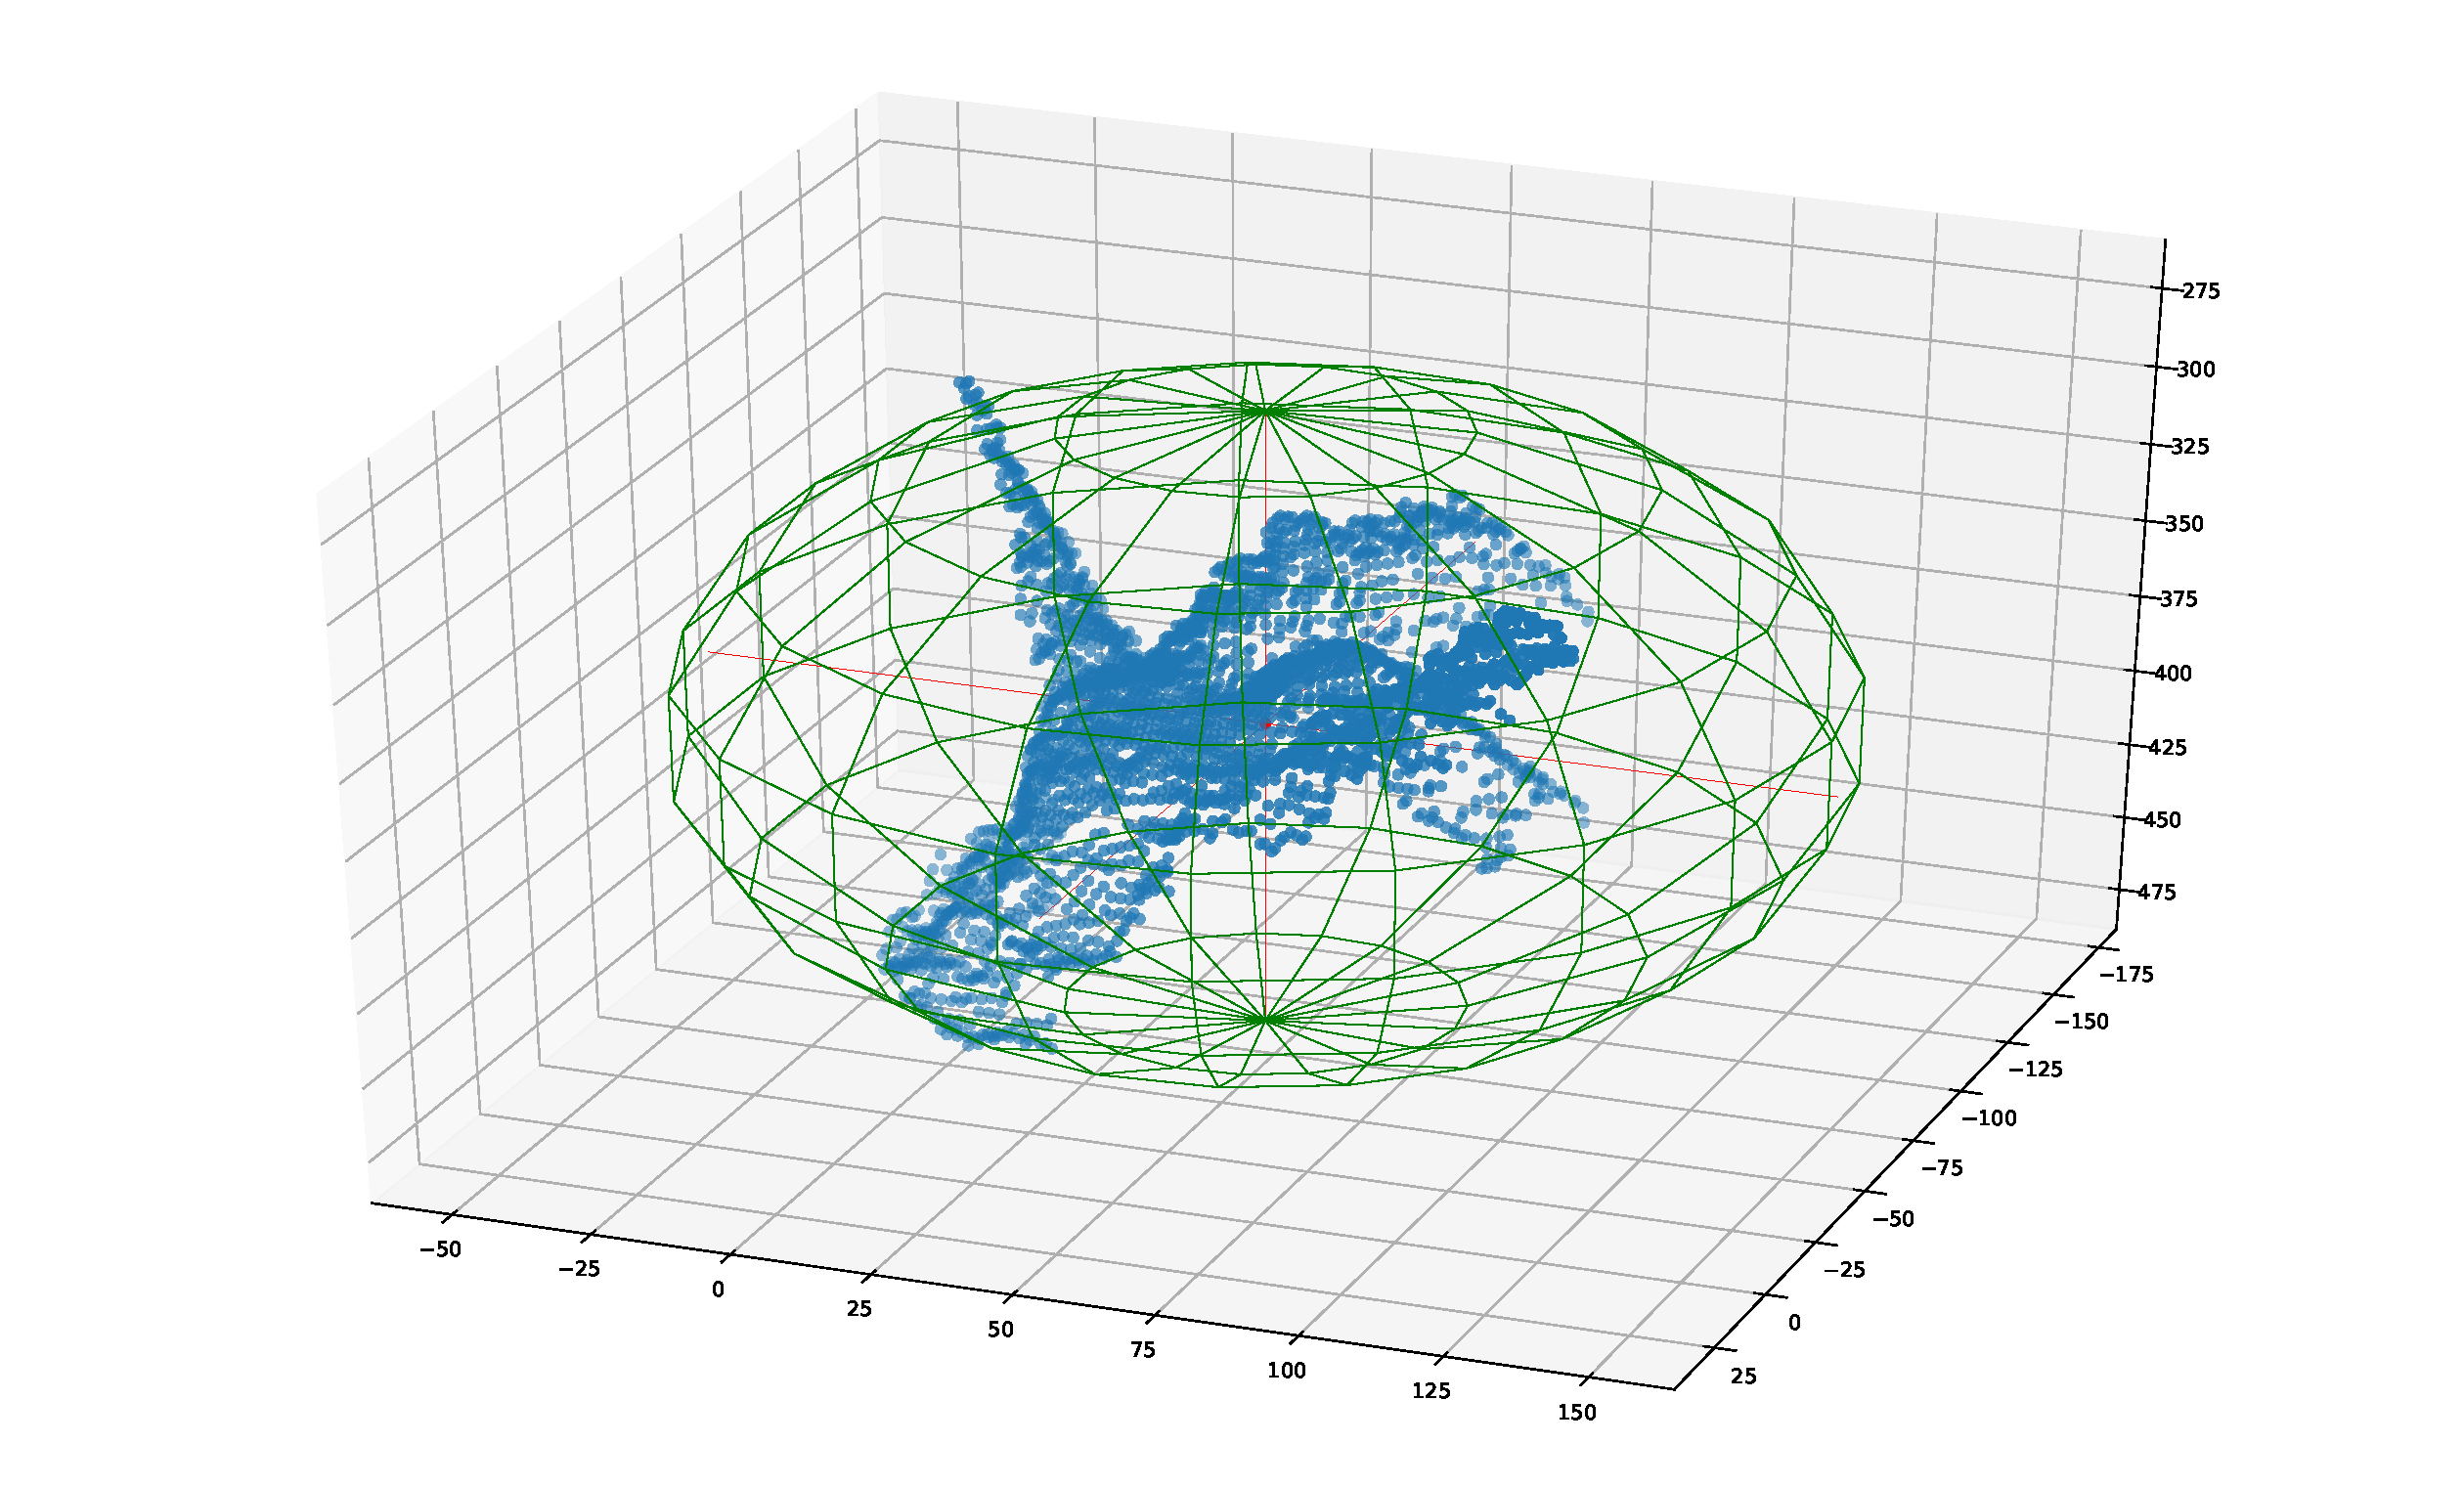
\includegraphics[width=0.5\linewidth]{figs/visualisation/pcloud0.pdf}
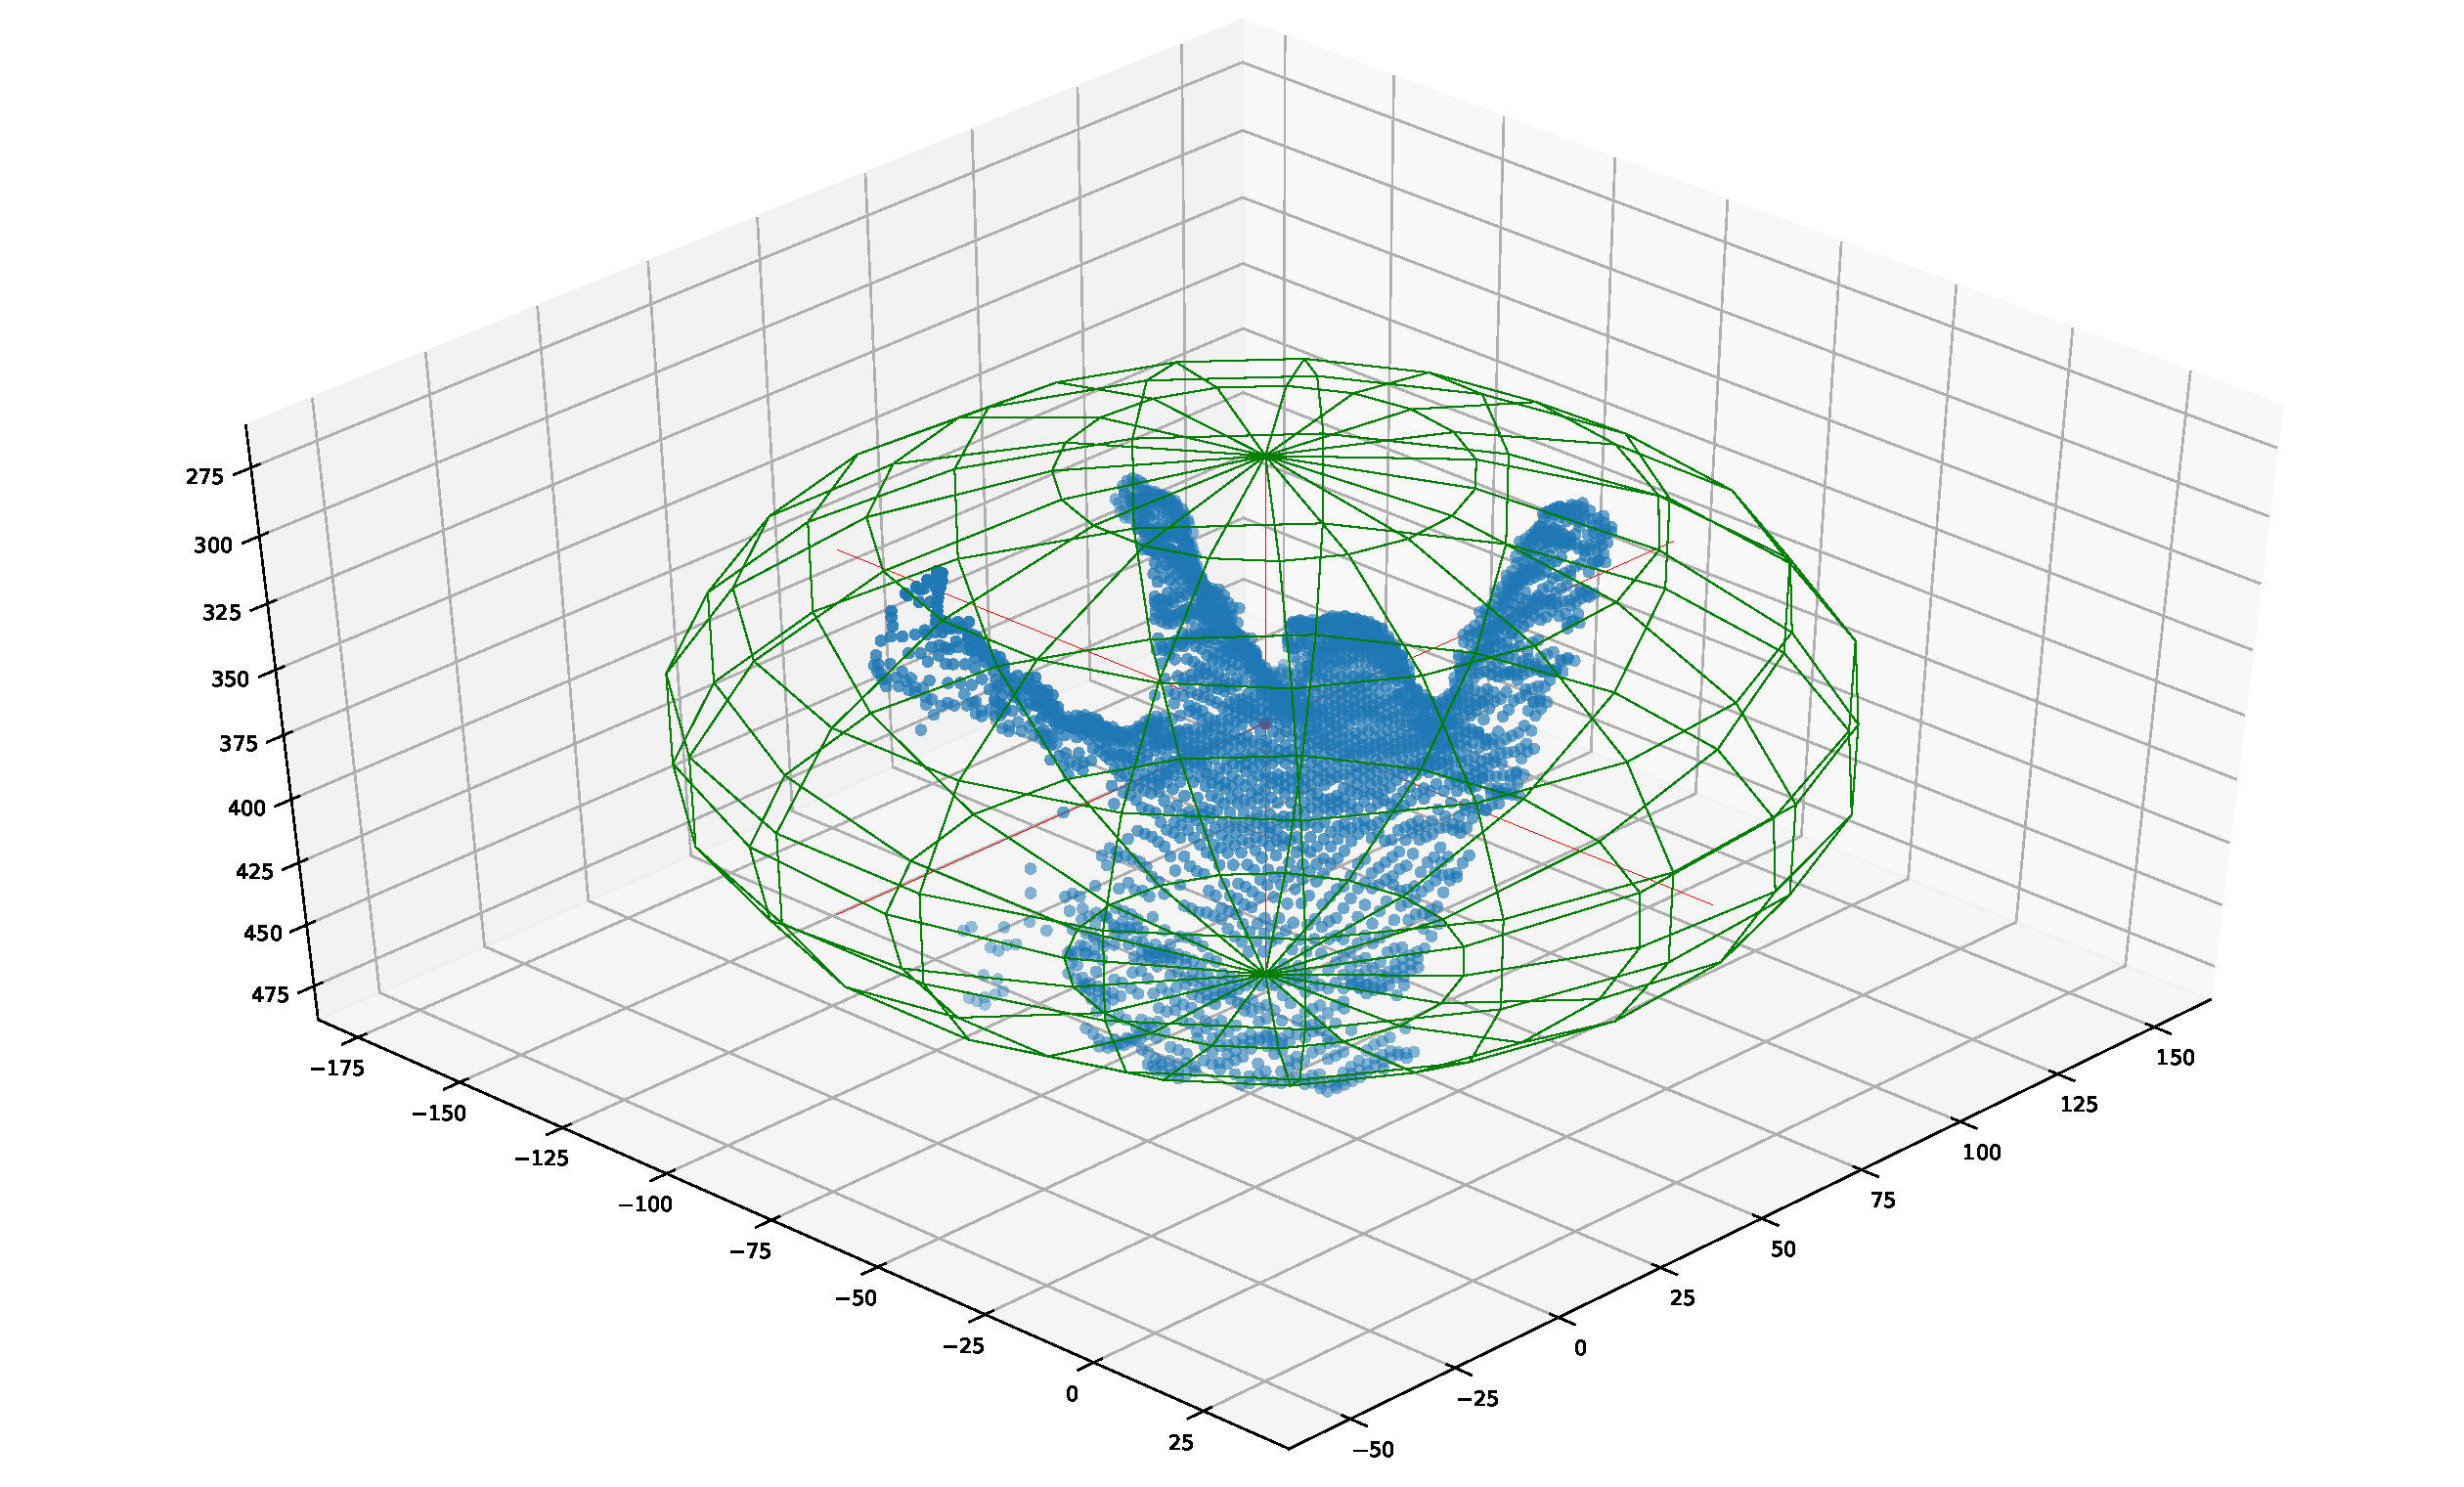
\includegraphics[width=0.5\linewidth]{figs/visualisation/pcloud1.pdf}
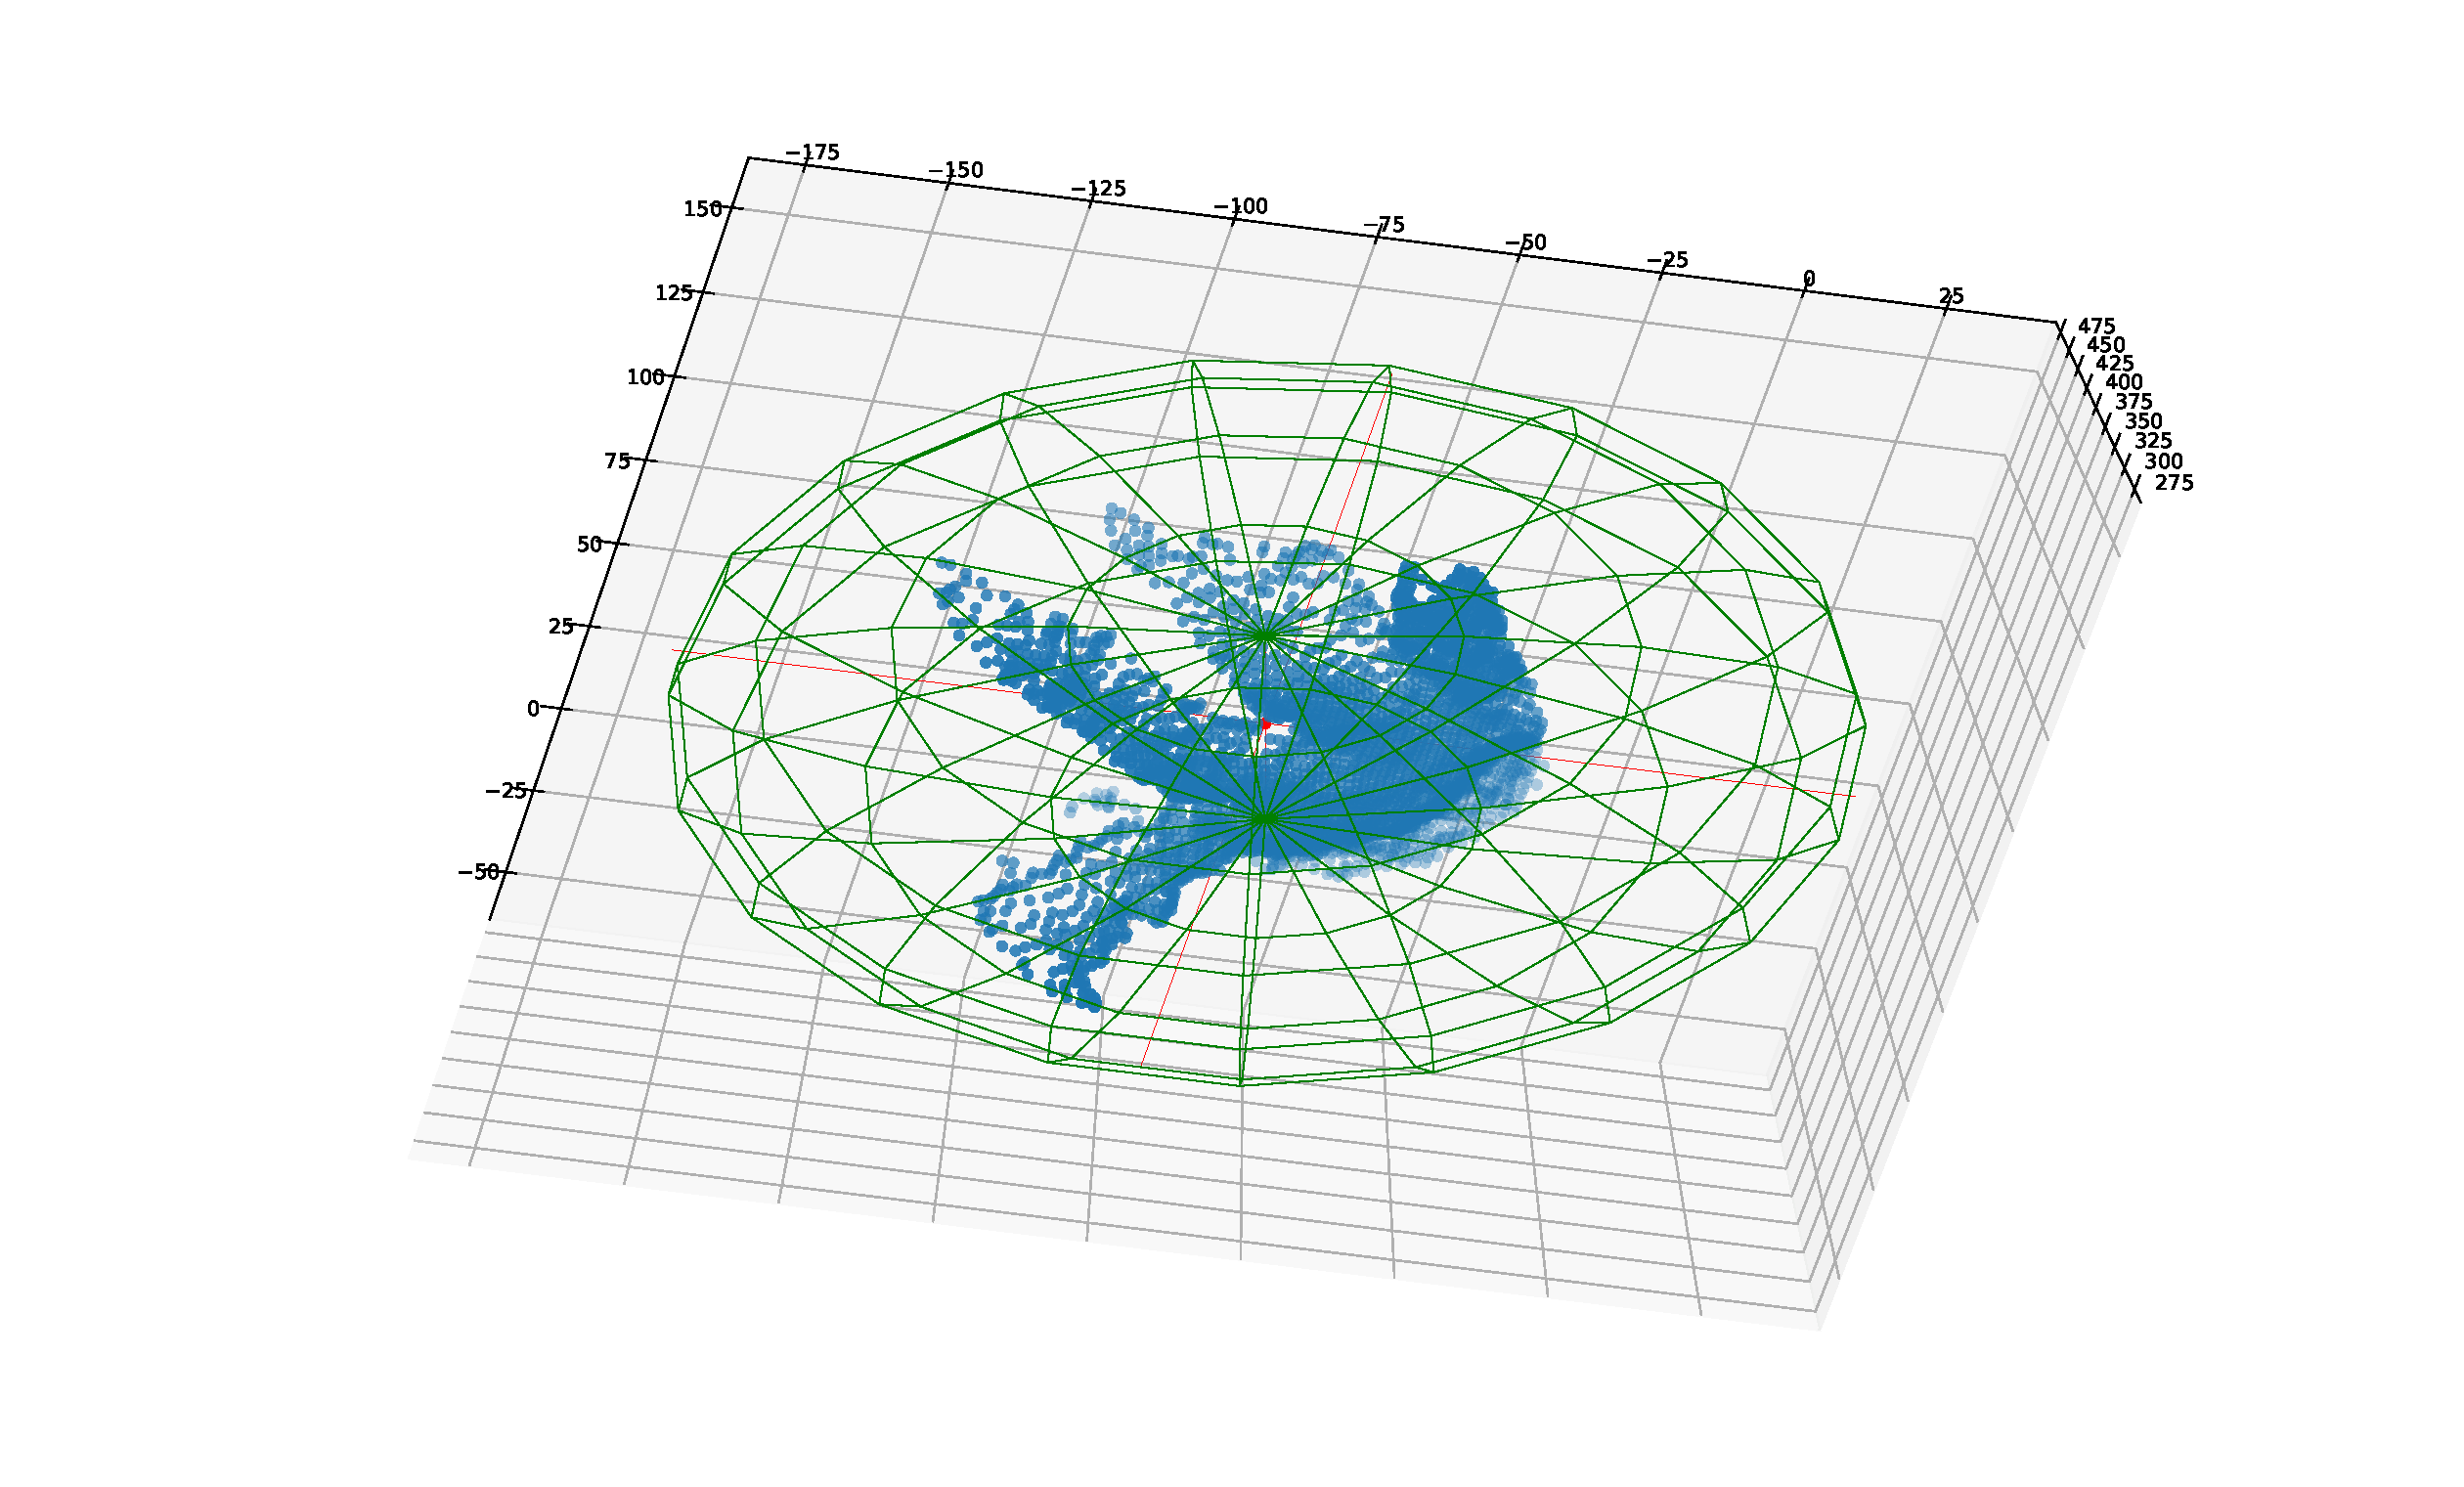
\includegraphics[width=0.5\linewidth]{figs/visualisation/pcloud2.pdf}
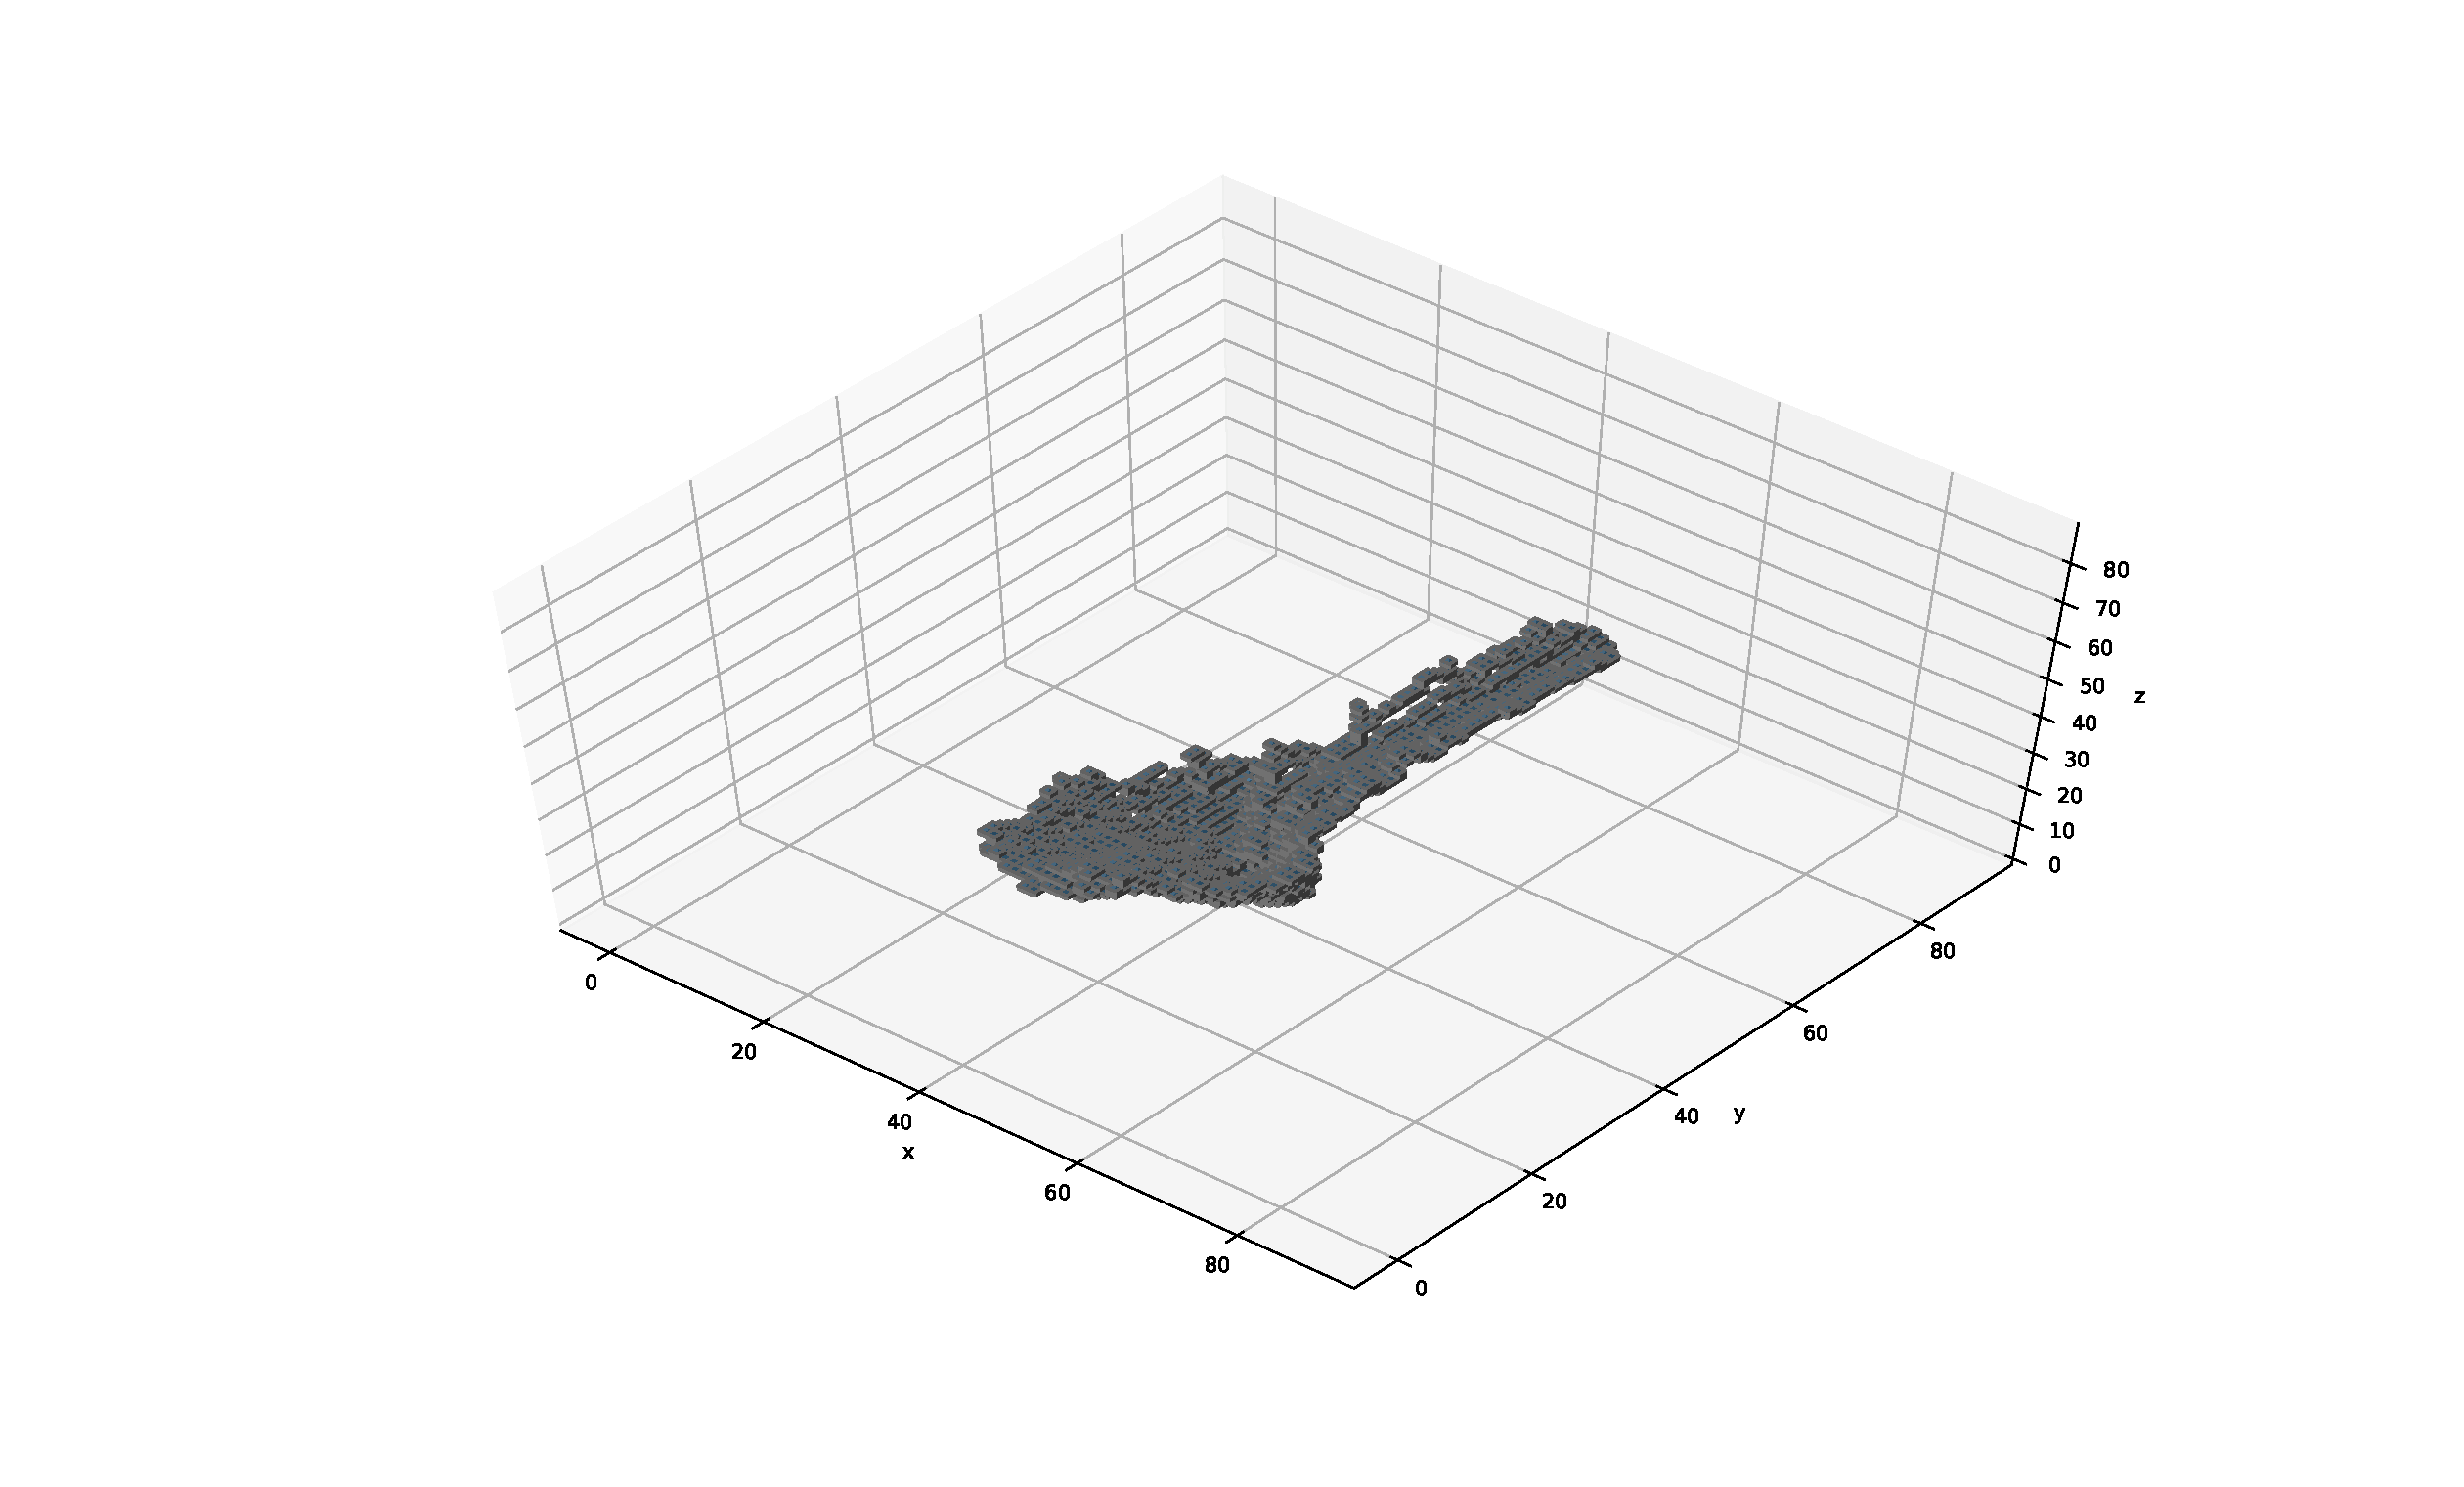
\includegraphics[width=0.5\linewidth]{figs/visualisation/vox0.pdf}
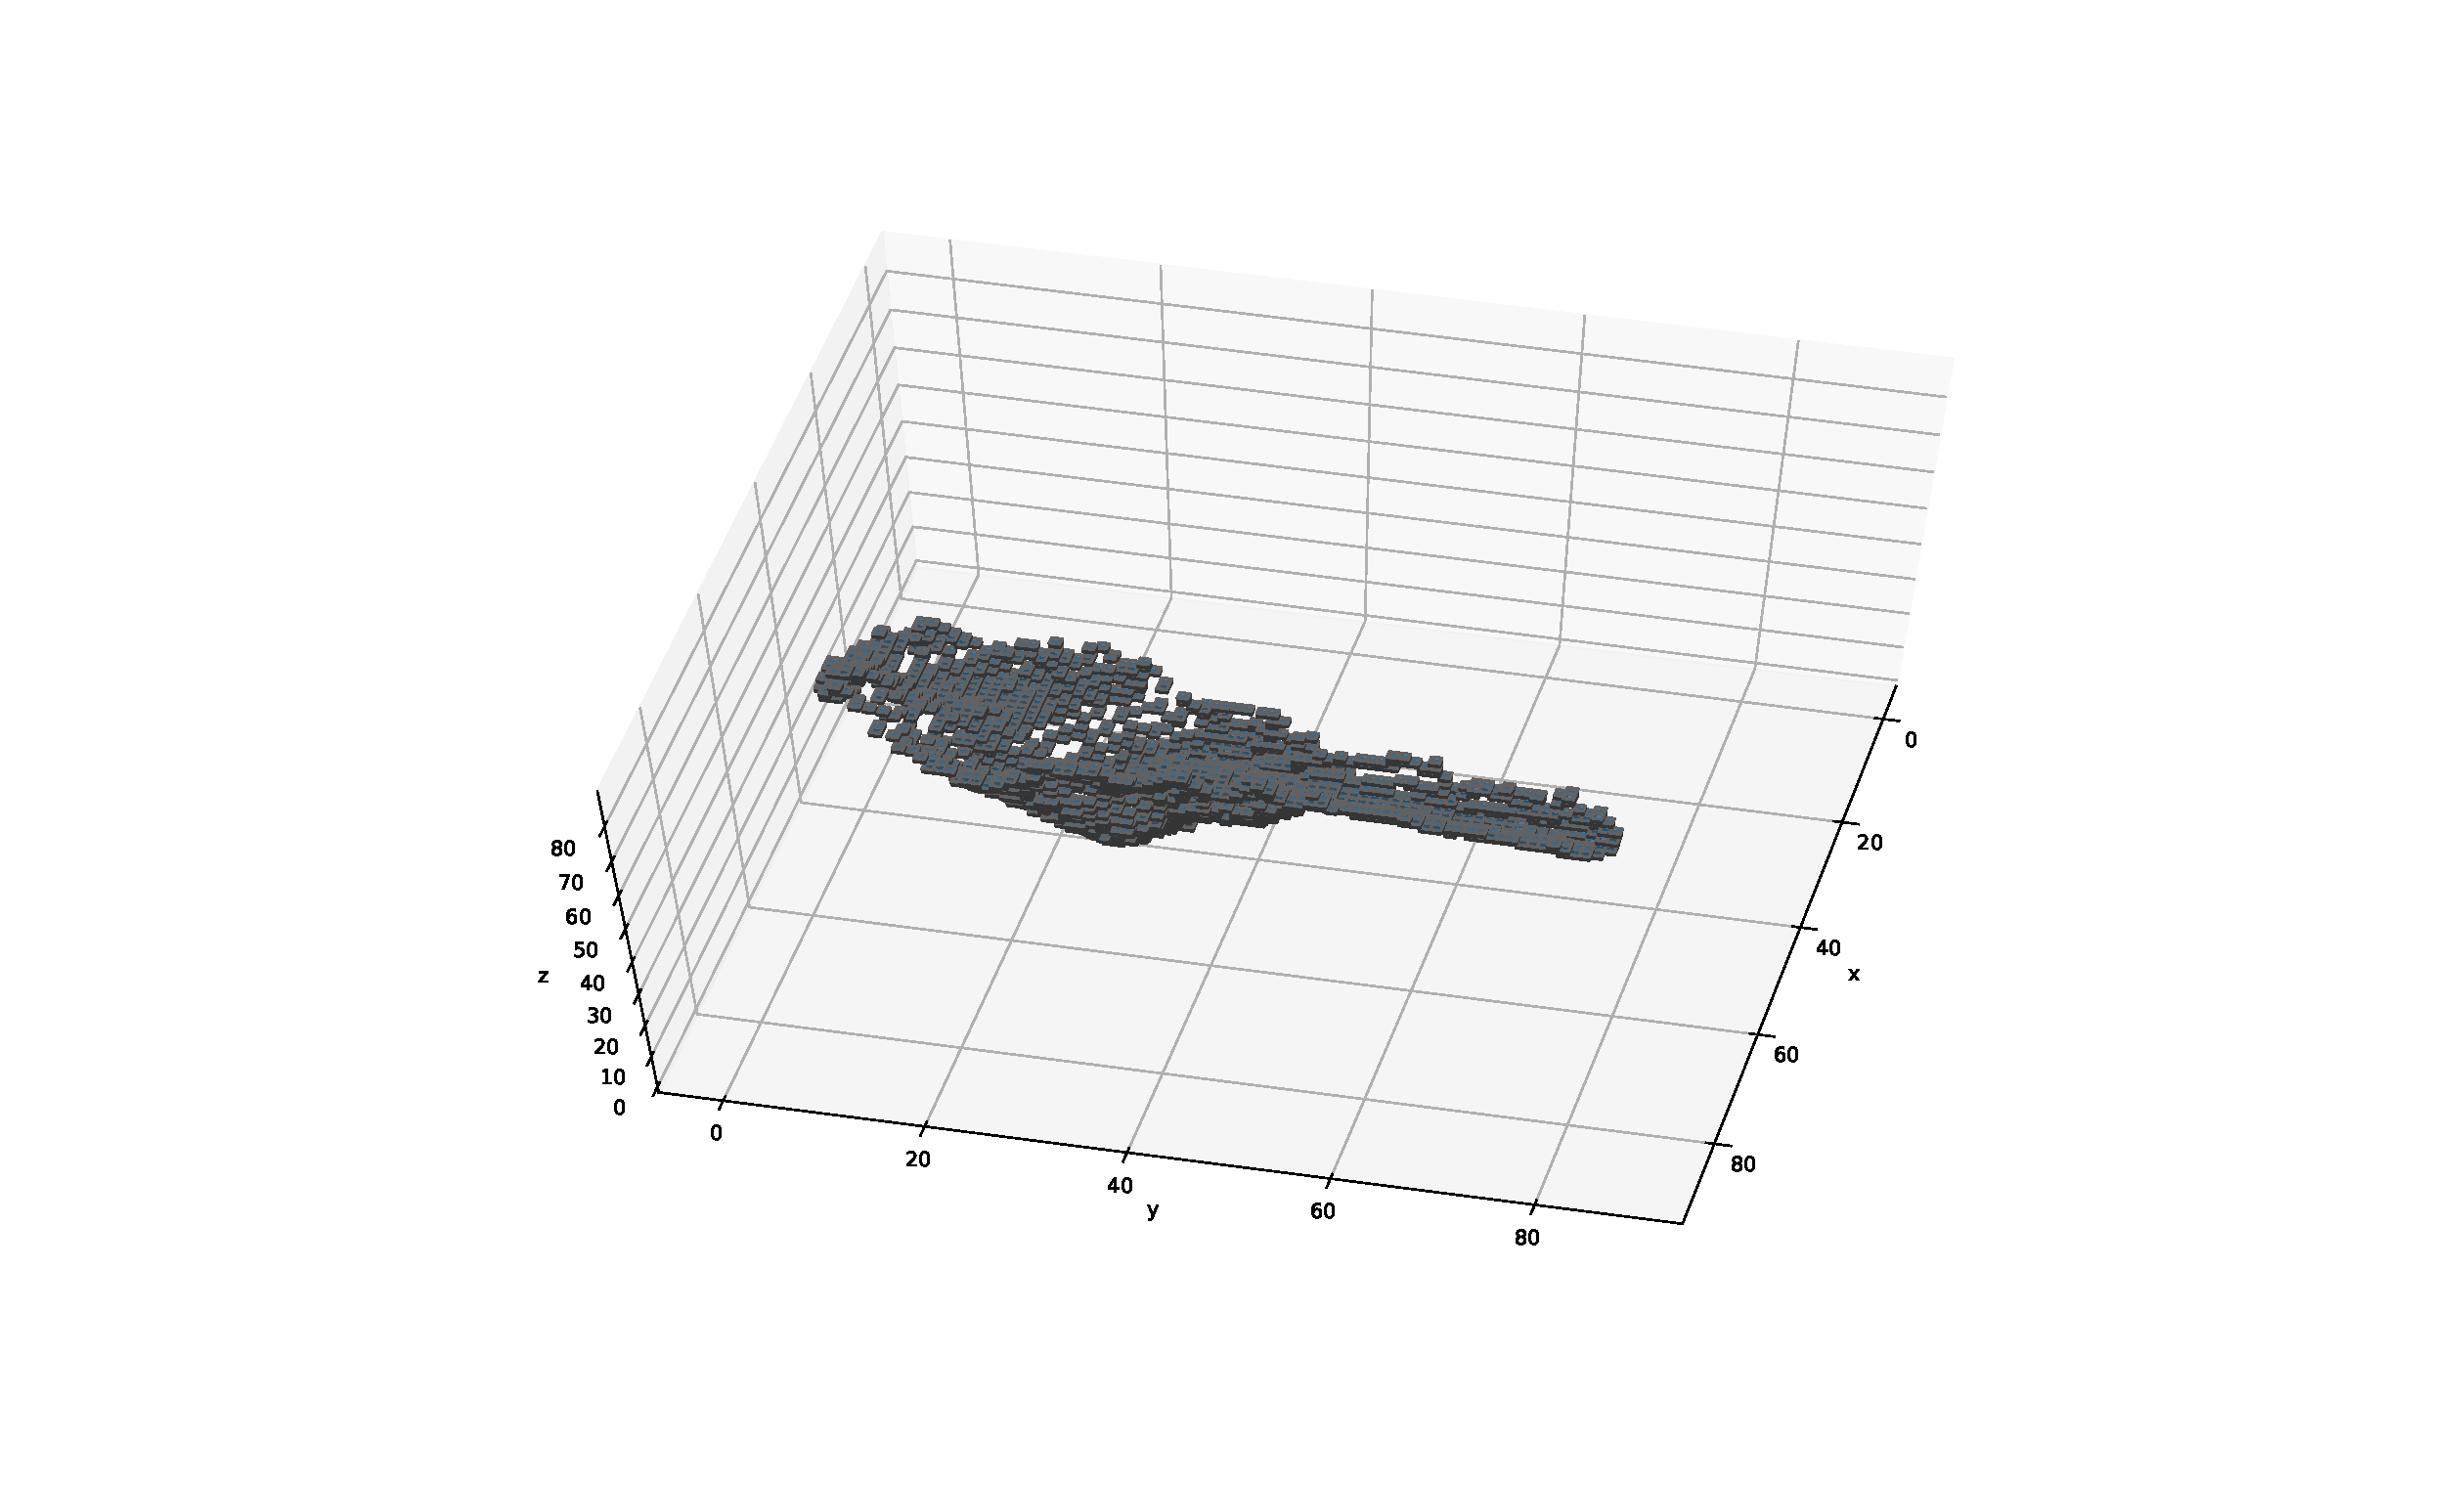
\includegraphics[width=0.5\linewidth]{figs/visualisation/vox1.pdf}
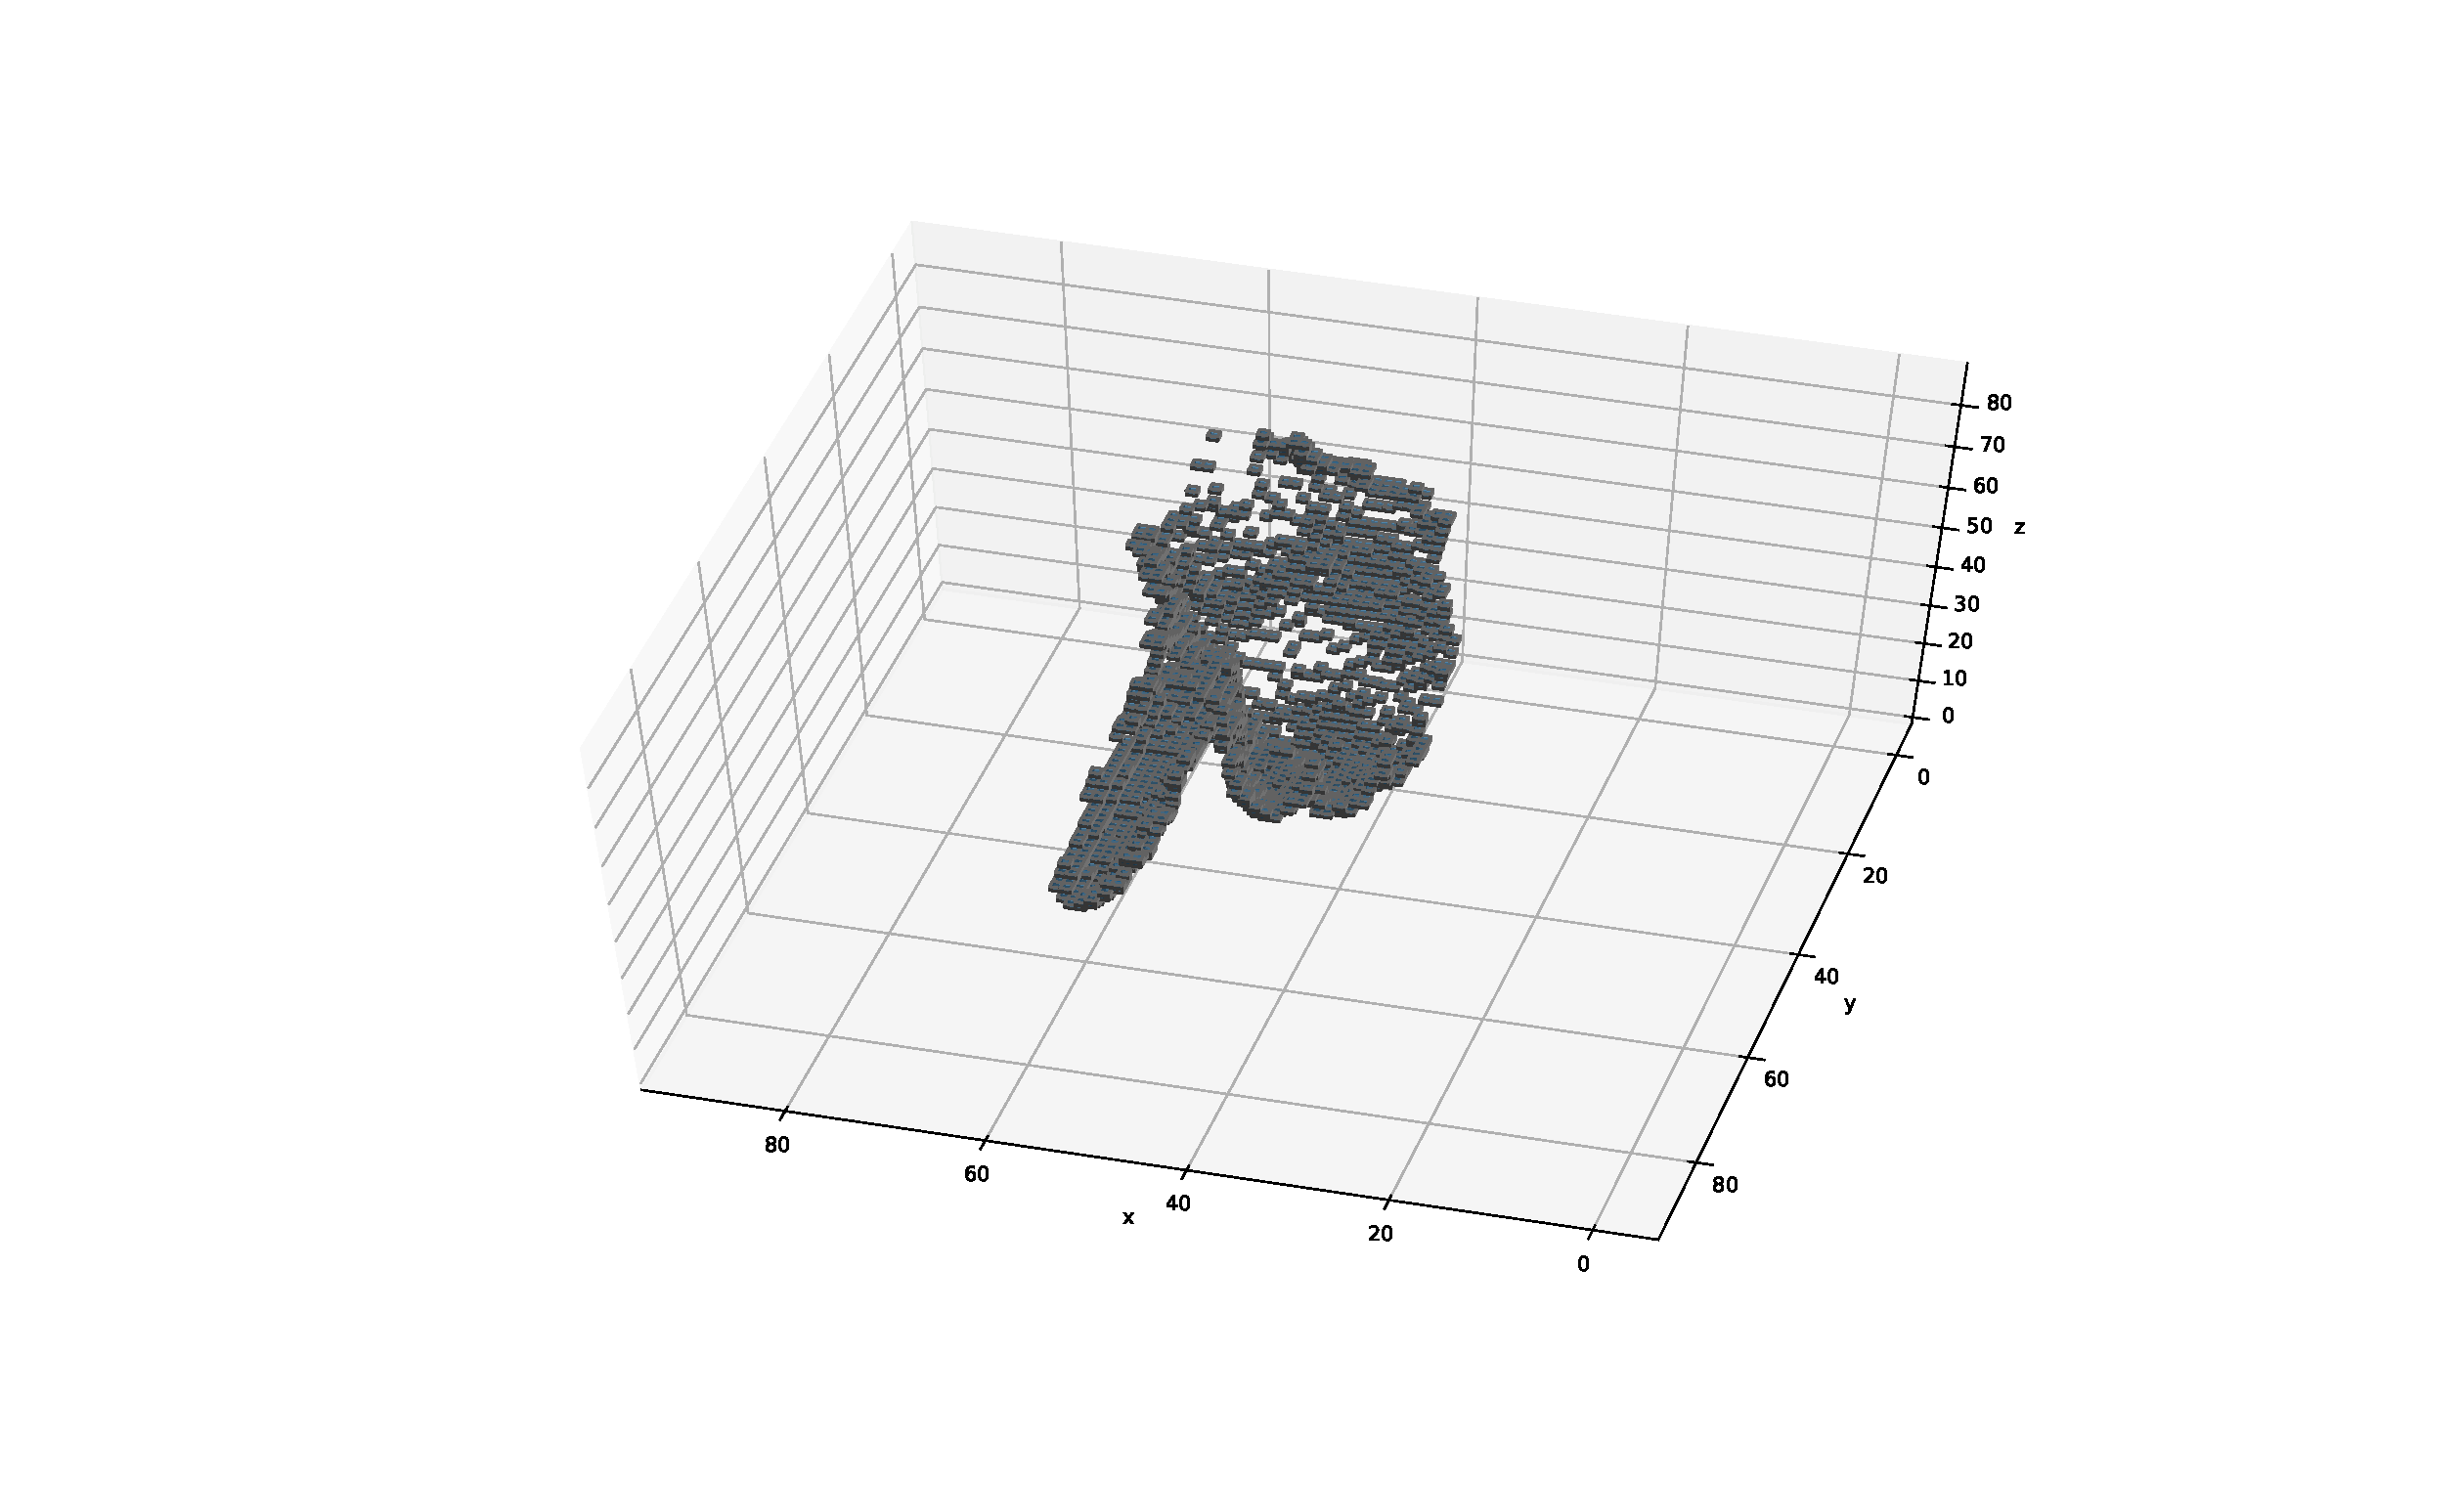
\includegraphics[width=0.5\linewidth]{figs/visualisation/vox2.pdf}
\caption{Examples the visualisation tools for the pointcloud (top row and middle left) and voxelisation (bottom row and middle right). For the pointcloud, all blue points that fall within the green sphere are voxelised, note as well that the background pixel points are not shown.}
\label{fig:es:pc}
\end{figure}

\subsubsection{Voxel Visualisation}
Converting from pointcloud to voxels is the last step in the pipeline before the data is passed to the V2V-Posenet model. This step is largely robust for a given pointcloud representation since it is part of the implementation of the V2V-Posenet model that is used for this dissertation. It does however serve to confirm that the pointcloud visualisation step itself works. This step also was implemented with {\slshape Matplotlib}. Examples are also in Figure \ref{fig:es:pc}.

% \begin{figure}
% 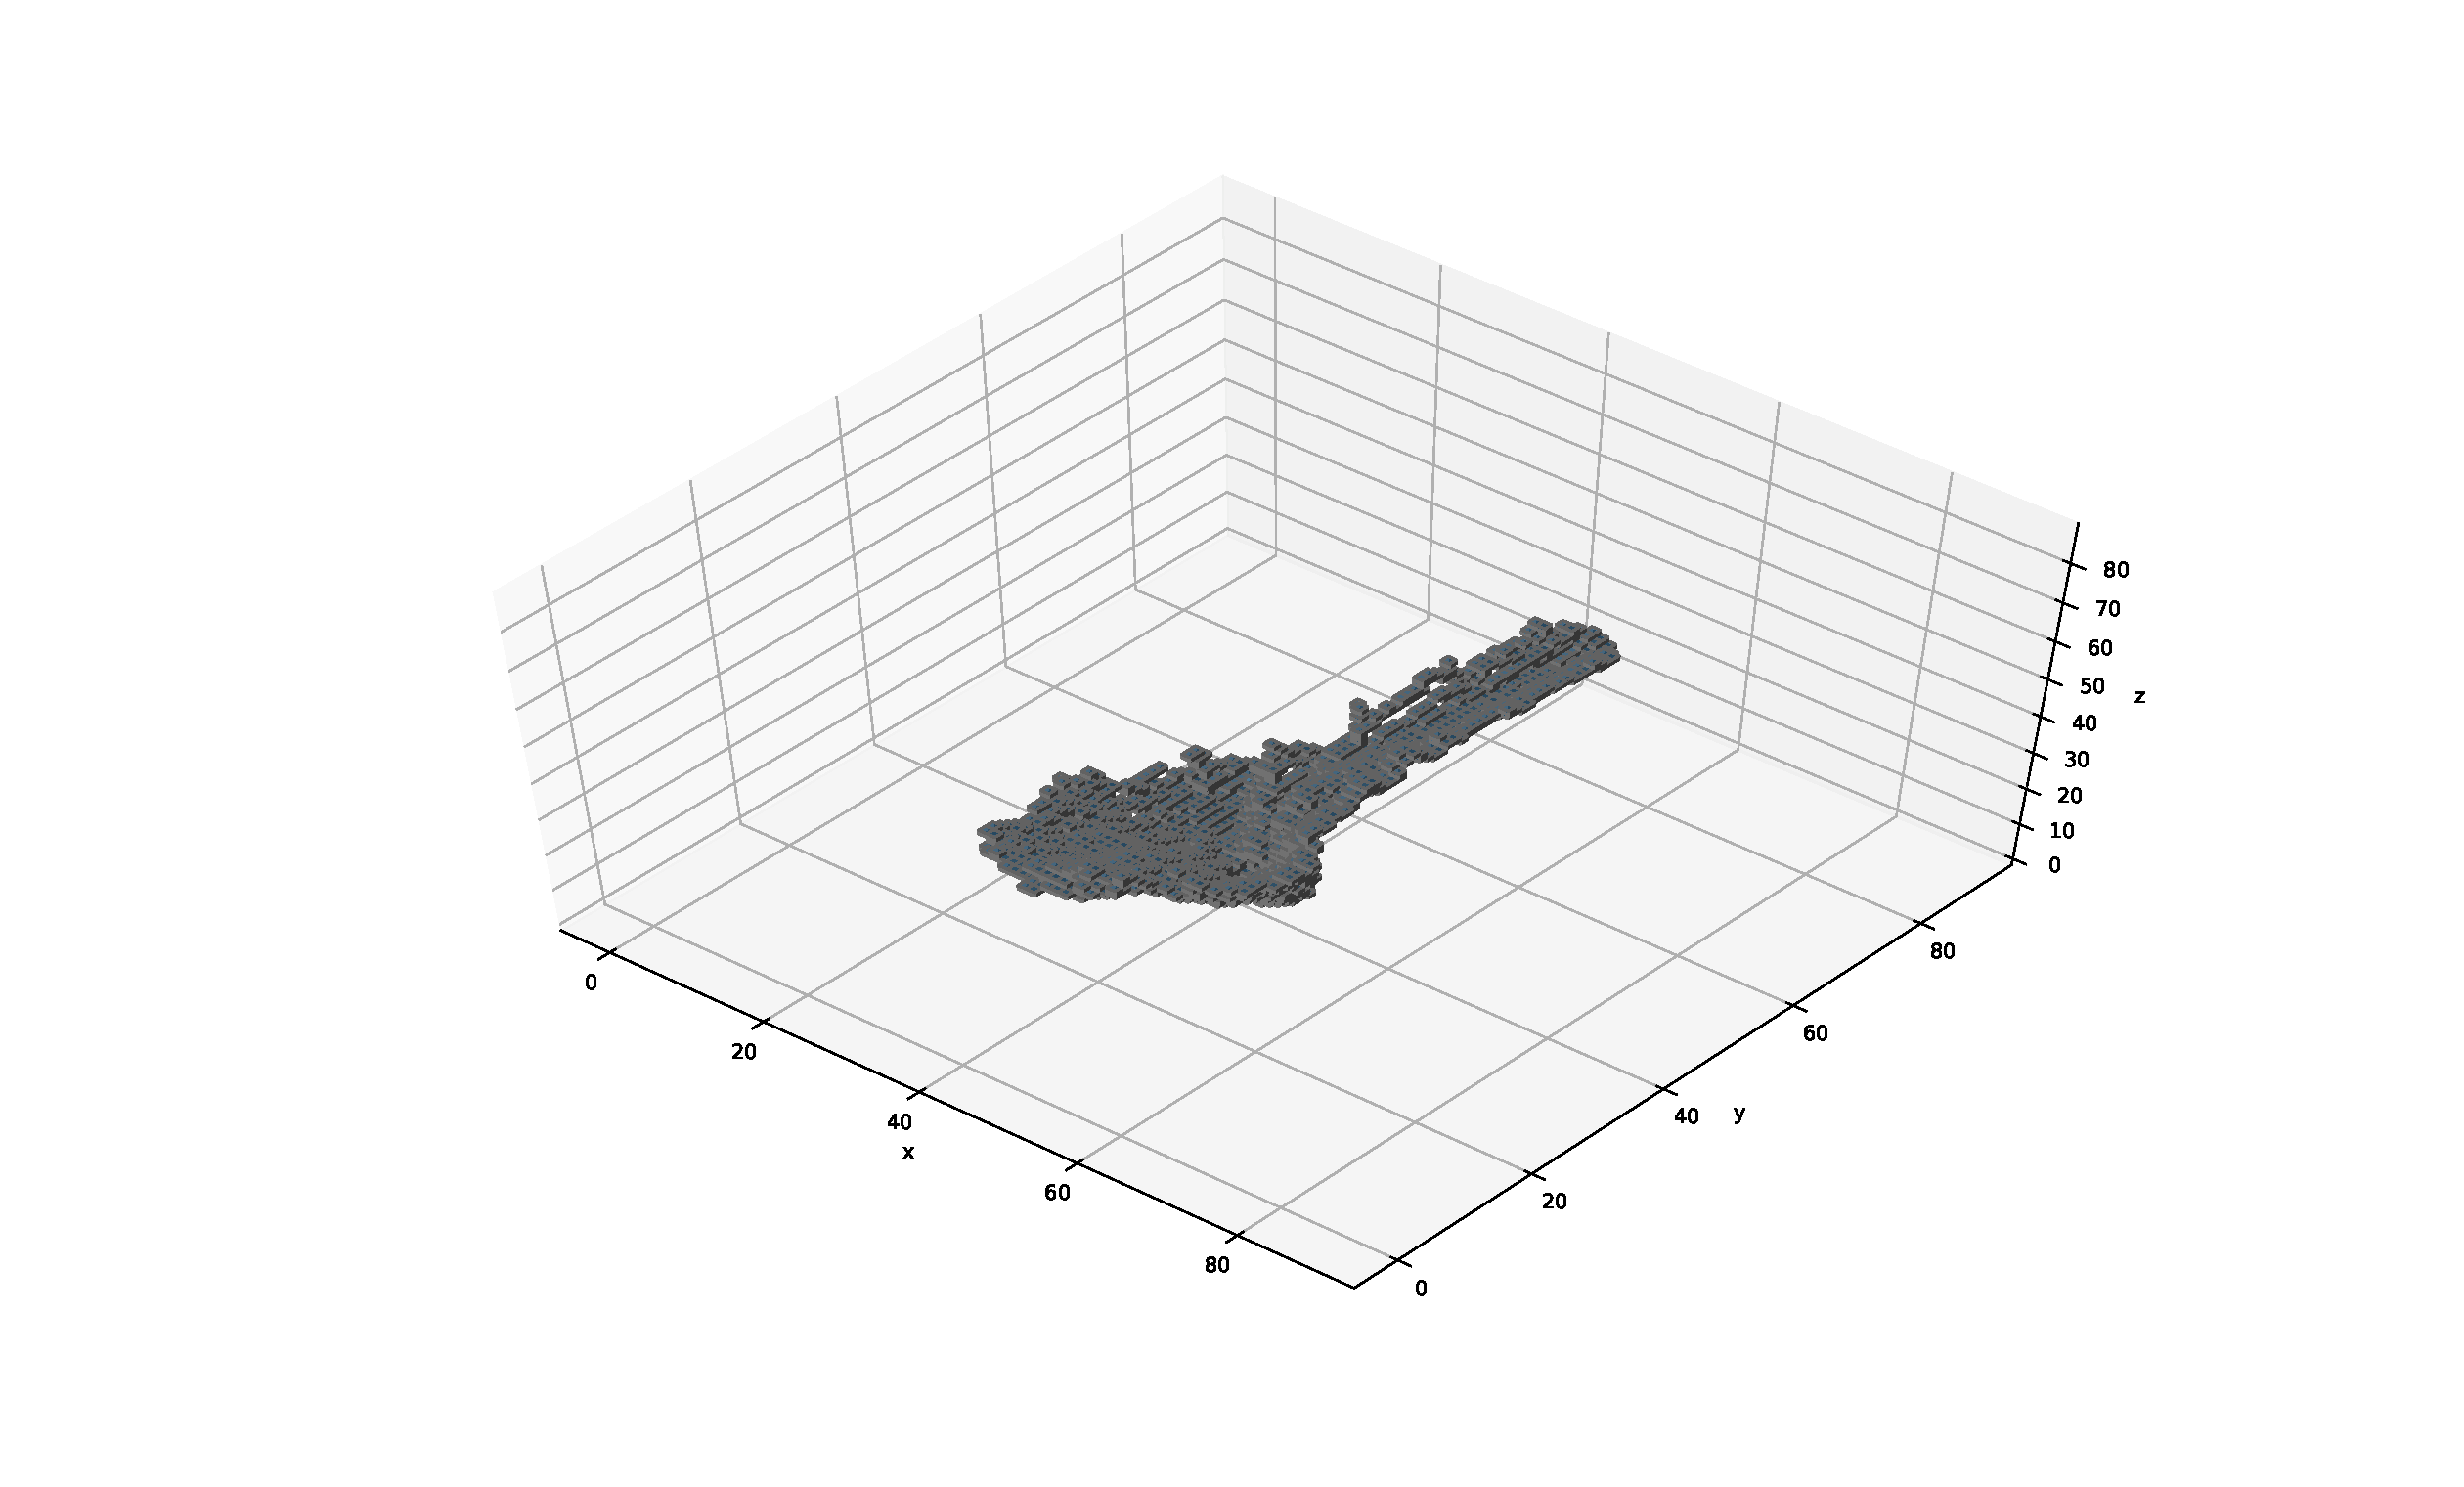
\includegraphics[width=140px]{figs/visualisation/vox0.png}
% 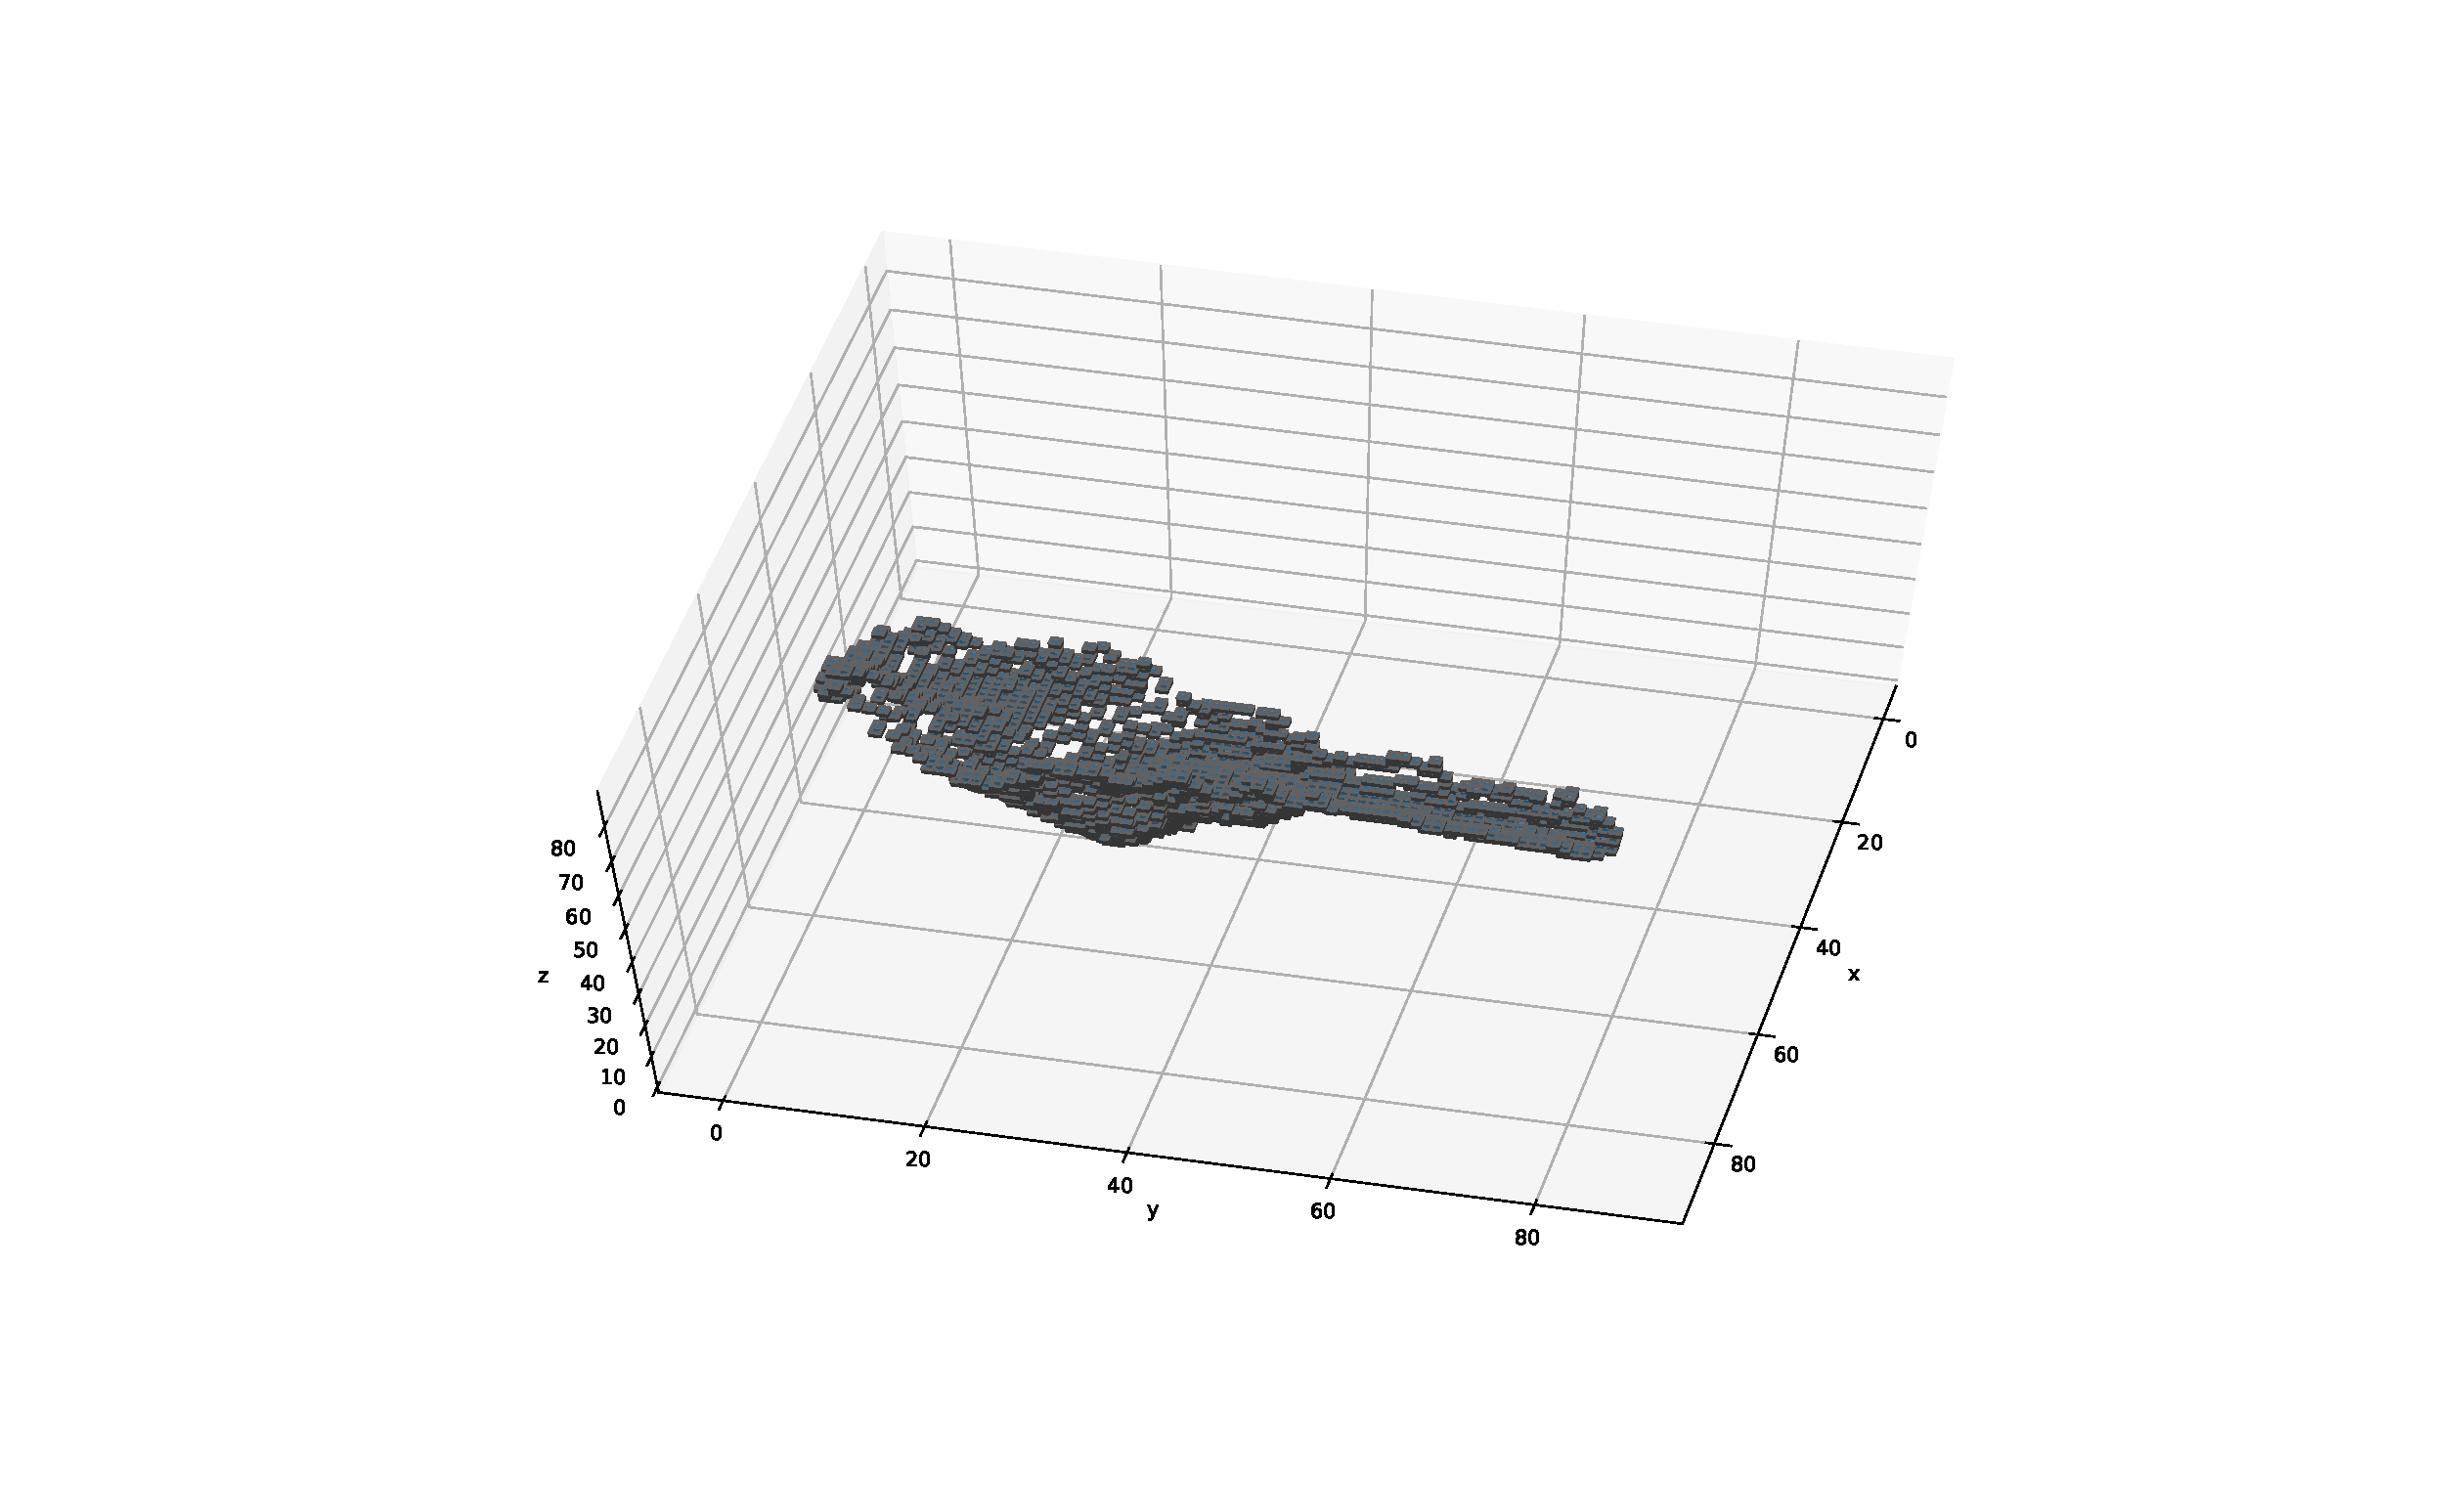
\includegraphics[width=140px]{figs/visualisation/vox1.png}
% 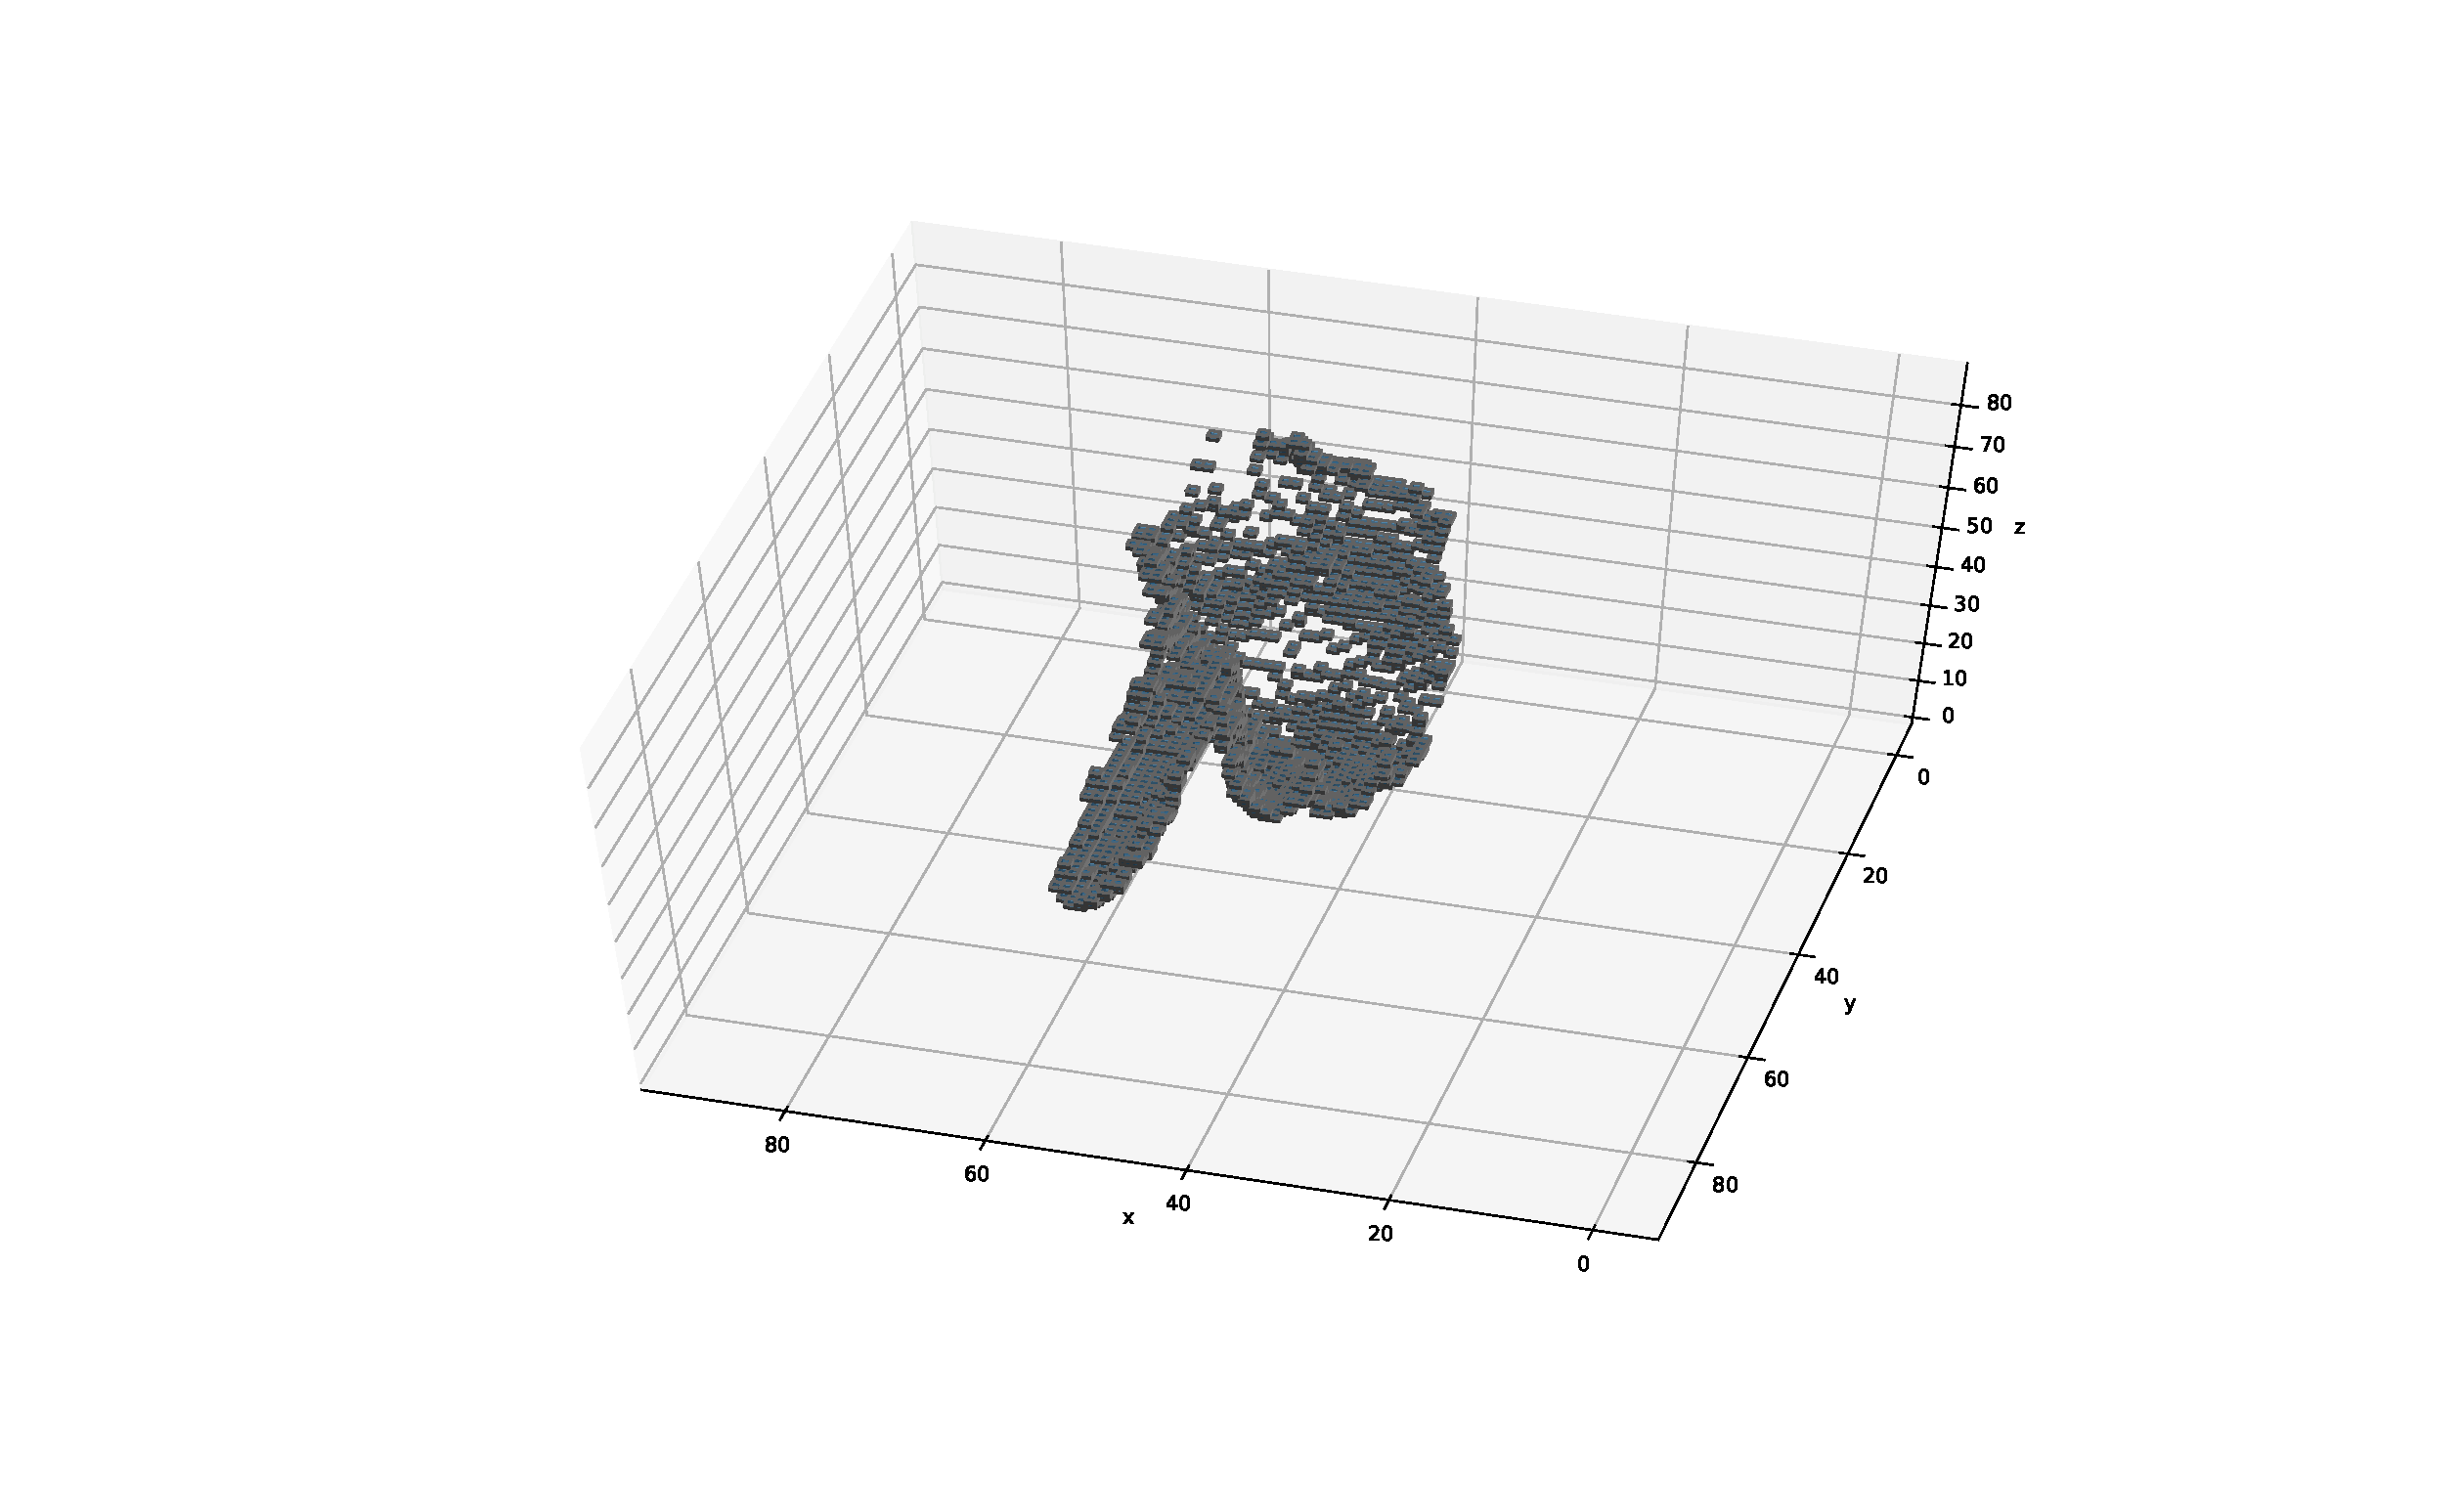
\includegraphics[width=140px]{figs/visualisation/vox2.png}
% \caption{Examples the visualisation tool for voxels from different perspectives, this uses the same input image used in Figure \ref{fig:es:pc}.}
% \label{fig:es:vox}
% \end{figure}

% To evaluate this, a simple metric of time is used. The overall time, as well as time per image is recorded. This became particularly important for rotations, I had previously used a liib


\section{Experiments}
\label{es:exp}
This section details the experiments undertaken in this dissertation. All experiments involved training the V2V-Posenet model for 5 epochs with a batch size of 12. Every dataset consists of 67893 training images, and 8498 test images.

\subsection{Baseline}
\label{es:ex:base}
The baseline of this dissertation is training the V2V-Posenet model with the real MSRA training dataset, it is then validated with the MSRA test dataset. It is also validated with the test datasets for the Random MANO and IK MANO datasets too.

\subsection{Analysis Of Synthetic Data}
The Random MANO and IK MANO datasets are investigated separately. Both respective training datasets are used to train the V2V-Posenet model under two scenarios; random initialisation of the V2V-Posenet weights, and one where the weights obtained from training the V2V-Posenet model on the MSRA training dataset are used as a base. In total, this gives four models obtained from training with synthetic data. Each of these four models are tested with the respective test synthetic dataset, and the MSRA test dataset, which gives eight testing scenarios. There are two error metrics described in Section \ref{sec:pm}, so this gives sixteen sets of results.

% As mentioned previously, the first experiment for this dissertation is training the V2V-Posenet model with the MSRA dataset to give a baseline. For both synthetic datasets, the V2V-Posenet model is then trained under two starting points, one where the weights of the V2V-Posenet model weights are initialised at random as is how the model is trained originally with the MSRA dataset, and one where the weights from the MSRA-trained baseline are used. In these four scenarios, the model is trained for five epochs as is the case for the baseline. For each training scenario, two testing scenarios are used. One where the test synthetic dataset is used against the performance metric, and one where the MSRA test dataset is used. In all, 16 sets of values are produced, which are summarised in Section \ref{chap:res}.

% \section{Maya}
% As previously mentioned, Maya \footnote{\url{https://autodesk.com/maya} (accessed 29th April 2020)} is the programme that was used to generate the synthetic dataset deterministically. In order for the problem to scale well, the process was entirely automated to the extent using the built-in Python implementation, which notably in the 2020 version uses version {\slshape 2.7.11}, which led to certain practical challenges using up-to-date libraries. As well as this, the generation of synthetic data had the ability to benefit from parallel execution, specifically when the render for a particular image was complete by Arnold, some further processing was required which could be done in parallel.

% \subsection{Execution Model}
% A producer-consumer execution model was used to achieve this, were the main programme, Maya Python spawns a child process using the \verb|subprocess.Popen| function call in the standard library. Very specifically, the \verb|subprocess.Popen| call is a wrapper for the {\slshape Fork-exec} technique. The {\slshape Fork-exec} technique is where a process creates a copy of itself using the \verb|fork()| call (available on all POSIX operating systems) which makes a clone of the parent process, so the child process has the replica, but seperate address space, and the same set of instructions, the two programmes can distinguish each other by the fact that \verb|fork()| returns the child's processor ID in the parent process, and zero in the child process. This is followed by the \verb|exec()| in the child process, which replaces the programme's machine instructions and address space with the new programme's, while keeping the same processor ID, and the parent continues with its own execution \footnote{\url{https://github.com/python/cpython/blob/master/Modules/_posixsubprocess.c} (accessed 29th April 2020)}.

% The child process runs a modern version of Python to perform the post-processing of each depth image. The parent and child processes communicate using a pipeline. Every time a new image is rendered in Maya, it saves the file to disk, when this occurs, the name, path, and grountruth of that image are passed to the child process in the pipeline, and the child performs the processing based on this information. In the execution pattern of the child, it waits for this information to be given to it. In order to strive towards deterministic execution, a \verb|SIGALARM| is set to check a boolean that says whether the programme should stop when waiting for input, and if it receives nothing in the next three seconds, and that boolean is set to true, the child process stops. In the parent process, a wrapper class for calling the child process is implemented, and when that wrapper class is garbage-collected, it send a \verb|SIGTERM| signal to the child, in the child, this sets the boolean to true, and if it is in the middle of processing an image, it will complete that first, and it will continue to process whatever is still in the pipeline before stopping.

\section{Miscellaneous}
\label{sec:sd:misc}
\subsection{Execution Model}
\subsubsection{}{Random MANO Dataset}
The MANO parameters $\bm{\beta}$ and $\bm{\theta}$ are determined at random for generating the Random MANO dataset. To make the generation of the data is made consistent over different runs, the random number generator is seeded with a constant value. When training, the images are generated at runtime before the model is trained and are stored in a temporary directory using the {\slshape tempfile} library\footnote{\url{https://docs.python.org/3.7/library/tempfile.html} (accessed 29th April 2020)} in Python. To give a fair comparison with the MSRA dataset, the same size for the training and test sets are used at 67893 and 8498 respectively. A different seed for the random number generator is used for training and testing. 

\subsubsection{IK MANO Dataset}
As previously mentioned, recreating the real dataset is achieved in Maya\footnote{\url{https://autodesk.com/maya} (accessed 29th April 2020)}, a 3D computer graphics programme. The actual renderer used is Arnold\footnote{\url{https://www.arnoldrenderer.com} (accessed 29th April 2020)}. This was running on a different computer to the one used to run the V2V-Posenet model, and it lacked a GPU which meant that it was not feasible to generate the dataset in real time with training the model (it takes 12 hours and 53 minutes to generate the training and test dataset, or 607 milliseconds per image). Given the size of the dataset, the process was scripted. Maya comes with a Python environment for writing scripts which has API calls for scripting tasks within Maya. An important implication of using Maya Python is that it uses Python 2.7.11, which was released in December 2015 and lacks the support of many modern libraries. As well as this, it does not come with {\slshape PIP}, a common package manager in Python, which made it more challenging to use certain third party libraries. As a way around this problem, as well as to make the execution of the programme more efficient, two processes were used in the synthetic data generation process; Maya Python, as well as another process running Python 3. This was achieved using the {\slshape subprocess} library in Python\footnote{\url{https://docs.python.org/release/2.7.11/library/subprocess.html} (accessed 29th April 2020)}.

The calculation of the camera position, hand articulation, as well as the rendering happend within the Maya Python process. The Python 3 process did extra processing on the image (using the Python {\slshape subprocess} library), this consisted of normalising the rendered images, then compressing them to save disk space (using the numpy.savez\footnote{\url{https://numpy.org/devdocs/reference/generated/numpy.savez.html} (accessed 29th April 2020)} method). The execution of these processes worked in a producer-consumer model. The child process runs a modern version of Python to perform the post-processing of each depth image. The parent and child processes communicate using a Unix-style pipeline. Every time a new image is rendered in Maya, it saves the file to disk, when this occurs, the name, path, and grountruth of that image are passed to the child process in the pipeline, and the child performs the processing based on this information. In the execution pattern of the child, it waits for this information to be given to it. In order to strive towards deterministic execution, a \verb|SIGALARM| is set to check a boolean that says whether the programme should stop when waiting for input, and if it receives nothing in the next three seconds, and that boolean is set to true, the child process stops. In the parent process, a wrapper class for calling the child process is implemented, and when that wrapper class is garbage-collected, it send a \verb|SIGTERM| signal to the child, in the child, this sets the boolean to true, and if it is in the middle of processing an image, it will complete that first, and it will continue to process whatever is still in the pipeline before stopping.

\subsection{Execution Speed}
Execution speed refers to how quickly the synthetic data pipeline can execute, from generating, processing, training, and testing on the synthetic data. While this is not necessarily needed in terms of ensuring that the synthetic data pipeline is optimal towards improving the performance metric, it is important towards improving the speed of the pipeline itself, since it means that less time can wasted between per development cycle. Since the software for this dissertation was written in Python, this primarily focussed on the optimal use of libraries within Python. Python is an Interpreted language, and is not compiled to machine code before execution so code written in it executes slowly in comparison to software that is compiled (such as C, C++ and Fortran). Some libraries in Python are written in compiled languages however. This means therefore that Python code should aim to offset as many instructions within the code to libraries that are written in compiled languages as possible.

\subsection{Computers}
Two computers were used in the experiments. The rational behind this is that one computer had a GPU which is needed for modern CNN training tasks, but it was not portable and lacked a GUI, a laptop was also used. The first computer, which was used for data visualisation and generating the MSRA-based synthetic dataset with Maya ran using a 2.6 GHz 6-core Intel i7 8850H, with 16GB of 2400MHz DDR4 RAM running macOS 10.15.3. The second computer used for the rest of the tasks in this dissertation used a 3.6 GHz 6-core AMD Ryzen 5 3600 with 32GB of 2400MHz DDR4 RAM and an Nvidia RTX 2060S with 8GB of GDDR6 RAM, running Ubuntu Server 18.04 LTS.

Since two computers were used for this dissertation, a practical concern during this project was how to communicate between the two computers. {\slshape Secure shell} (SSH) proved to be the most useful tool to achieve this. The internet connection for the server does not allow for port forwarding, which means that it cannot be an SSH server that is accessible from the internet. To solve this problem, a VPN server was deployed on Amazon Web Services (AWS). The AWS-based VPN server had a permanent connection to this computer, so when an SSH connection was made to the server from my laptop, it connected via this VPN server. Given the nature of this project, large quantities of data transfer were required, and AWS charges for this beyond a threshold, so the server did not connect to the internet via the VPN save for SSH communication. For the data visualisation tasks described in Section \ref{sec:es:st:dv}, the programme in the server interacts at different stages of the V2V-Posenet pipeline to extract information, and writes this data as a Python script, which can be copy and pasted onto my laptop. Given the small file size, this proved to be computationally feasible. 